%% LaTeX Paper Template, Flip Tanedo (flip.tanedo@ucr.edu)
%% GitHub: https://github.com/fliptanedo/paper-template-2022

% \documentclass[11pt]{article} %% Not for Lecture Notes
\documentclass[12pt, oneside]{report}    %% Has chapters

%!TEX root = lecturenotes.tex
%% Macros for lecture note typesettingj
%% Needs to be loaded before FlipPreamble.tex

%%%%%%%%%%%%%%%%%%%%%%%%%%%%%%%%%%%%%
%% BibLaTeX for footnote citations %%
%%%%%%%%%%%%%%%%%%%%%%%%%%%%%%%%%%%%%

%% BibLaTeX does not want the cite package
%% from: https://tex.stackexchange.com/a/39418/8094
\makeatletter
\newcommand{\disablepackage}[2]{%
  \disable@package@load{#1}{#2}%
}
\newcommand{\reenablepackage}[1]{%
  \reenable@package@load{#1}%
}
\makeatother

%% The following line prevents cite from being loaded
\disablepackage{cite}{}

%% We use biblatex for footnote citations
\usepackage[utf8]{inputenc}     % inspire bibs, load before biblatex
\disablepackage{inputenc}{}		% disable in preamble (double loading)
\usepackage[style=verbose]{biblatex}
% In main tex file
% \addbibresource{FlipBib.bib}


%%%%%%%%%%%%%%%%%%%%%%%%%%%%%%%%%
%% Package for making an index %%
%%%%%%%%%%%%%%%%%%%%%%%%%%%%%%%%%

\usepackage{makeidx}		% For index
\makeindex

%% Use \printindex command


%%%%%%%%%%%%%%%%%%%%%%%%%%%%%%%%%%%%%
%% SIDE NOTES AND RELATED COMMANDS %%
%%%%%%%%%%%%%%%%%%%%%%%%%%%%%%%%%%%%%

\usepackage{sidenotes}  
\renewcommand*\thesidenote{\alph{sidenote}}  %% sidenotes indexed letters

% Reset sidenote numbering
\let\oldchapter\chapter
\def\chapter{%
  \setcounter{sidenote}{1}%
  \oldchapter
}

%% Sidenote font and size
%% PART I: https://tex.stackexchange.com/a/536083/8094
%% n.b. a/532251/8094 broke the sidenote floating
    \usepackage{xparse}
    \let\oldmarginpar\marginpar
    \RenewDocumentCommand{\marginpar}{om}{%
      \IfNoValueTF{#1}
        {\oldmarginpar{\mymparsetup #2}}
        {\oldmarginpar[\mymparsetup #1]{\mymparsetup #2}}}

    \newcommand{\mymparsetup}{\scriptsize\sffamily}        % New, using xparse

    %% Old answer in a/532251/8094 makes all sidenotes marginnotes
    %% New answer (above) uses marginpar 
    % \renewcommand*{\marginfont}{\sffamily}    % Old
    % \renewcommand{\sidecaption}{\scriptsize\sffamily}

%% For marginnote font:
%% https://tex.stackexchange.com/questions/532245/how-to-modify-fonts-in-sidenotes/536083#536083
%% and see sidenotes documentation:
%% marginnote is a way to place notes with no mark
\renewcommand*{\marginfont}{\scriptsize\sffamily} 



%% Sans Serif Font Option for Sidenote
%% We use Sans Serif for captions and side notes. 
\usepackage[thin, scaled=1]{FiraSans} 
\DeclareCaptionStyle{sidecaption}{font={sf,footnotesize}}
\DeclareCaptionStyle{widefigure}{font={footnotesize,sf}}






%%%%%%%%%%%%%%%%%%%%%%%%%%%%%%%%%%
%% SILENCING Marginpar WARNINGS %%
%%%%%%%%%%%%%%%%%%%%%%%%%%%%%%%%%%
%% https://www.lucasshen.com/notes/tex-warnings/tex-warnings

\usepackage{silence}
\WarningFilter{latex}{Marginpar on page}
%% Silences: LaTeX Warning: Marginpar on page 1 moved.



%%%%%%%%%%%%%%%%%%%%%%%%%%%%%%%%%%
%% FORMATTING THE CHAPTER HEADER %%
%%%%%%%%%%%%%%%%%%%%%%%%%%%%%%%%%%
\usepackage{titlesec}
\titleformat{\chapter}[display]
  {\normalfont\sffamily\huge\bfseries\color{gray}}
  {\chaptertitlename\ \thechapter}{20pt}{\Huge\color{black}\textrm}
% \titleformat{\section}
%   {\normalfont\sffamily\Large\bfseries\color{cyan}}
%   {\thesection}{1em}{}



%%%%%%%%%%%%%%%%%%%%%%%%%%%%%%
%% FORMATTING THE PART PAGE %%
%%%%%%%%%%%%%%%%%%%%%%%%%%%%%%
% https://tex.stackexchange.com/a/202324
% Descriptive text after a Part is on the same page

\usepackage{xpatch}
\makeatletter
\xpatchcmd{\@endpart}{\vfil\newpage}{ \vspace{1em} }{}{}
\xpatchcmd{\@endpart}{\newpage}{}{}{}
\makeatother

       %% Lecture note formatting, load first
%!TEX root = paper.tex
%% FLIP’S PREAMBLE; 
%% Use FlipAdditionalHeader for project-specific packages & macros
%% Leave this as general as possible

%%%%%%%%%%%%%%%%%%%%%%%%%%
%%%  COMMON PACKAGES  %%%%
%%%%%%%%%%%%%%%%%%%%%%%%%%

\usepackage{amsmath}            % AMS Macros
\usepackage{amssymb}            %
\usepackage{amsfonts}           %
\usepackage{amsthm}             % 

\usepackage{graphicx}           % includegraphics
\usepackage[utf8]{inputenc}     % inspire bibs
\usepackage{aas_macros}				  % ADS bibs
\usepackage{bm}                 % \boldsymbol
\usepackage{microtype}          % improved typogarphy
\usepackage{etoolbox}           % LaTeX primitives

%%%%%%%%%%%%%%%%%%%%%%%%%%%
%%%  UNUSUAL PACKAGES  %%%%
%%%%%%%%%%%%%%%%%%%%%%%%%%%

%% MATH AND PHYSICS SYMBOLS
%% ------------------------
\usepackage{slashed}				% \slashed{k}
\usepackage{mathrsfs}				% Weinberg-esque letters
\usepackage{bbm}					  % \mathbbm{1} conflict: XeLaTeX 
\usepackage{cancel}					% cross out
\usepackage[normalem]{ulem} % for \sout
\usepackage{youngtab}	    	% Young Tableaux
\usepackage{mleftright}     % \mleft, \mright; bracket size/spacing

%% CONTENT FORMAT AND DESIGN
%% -------------------------
\usepackage[dvipsnames]{xcolor}
\usepackage[hang,flushmargin]{footmisc} % no footnote indent

\usepackage{fancyhdr}		% preprint number
\usepackage{lipsum}			% block of text 
% \usepackage{tcolorbox}  % replace framed and mdframed
\usepackage[most]{tcolorbox} % `most' needed for listings
\usepackage{subcaption}	% subfigures
\usepackage{cite}			  % group cites
\usepackage{wrapfig}    

%% TABLES IN LaTeX
%% ---------------
\usepackage{booktabs}		% professional tables
\usepackage{nicefrac}		% fractions in tables,
\usepackage{multirow}		% multirow elements in a table
\usepackage{arydshln}		% dashed lines in arrays

%% ARRAY STRETCH: vertical spacing between rows
% \renewcommand{\arraystretch}{1.5} %% put this in main text

%% Other Packages and Notes
%% ------------------------
\usepackage[font=small]{caption} 	% caption font is small
\usepackage{float}         			  % for strict placement e.g. [H]
\usepackage{lineno}               % Line numbers (put \linenumbers in main text)
\usepackage{ccicons}              % Creative Commons License Icons

%%%%%%%%%%%%%%%%%%%%%%%%%%%%%%
%%%  DOCUMENT PROPERTIES  %%%%
%%%%%%%%%%%%%%%%%%%%%%%%%%%%%%

\usepackage[margin=2.5cm]{geometry} % margins
\usepackage{changepage}             % overwrite geometry (e.g. lecturenotes)
\numberwithin{equation}{section}    % set equation numbering
\usepackage{marginnote}             % for \marginnote{comment}
% \usepackage{mparhack}               % fix for \marginnote
% \usepackage{marginfix}              % fix for \marginnote
% \usepackage{adjustbox}              % to rescale elements

%% References in two columns, smaller
%% http://tex.stackexchange.com/questions/20758/
\usepackage{multicol}
% \usepackage{etoolbox} %% called above
\usepackage{relsize}
\patchcmd{\thebibliography}
  {\list}
  {\begin{multicols}{2}\smaller\list}
  {}
  {}
\appto{\endthebibliography}{\end{multicols}}

% Change list spacing (instead of package paralist)
% from: http://en.wikibooks.org/wiki/LaTeX/List_Structures#Line_spacing
% alternative: enumitem package
\let\oldenumerate\enumerate
\renewcommand{\enumerate}{
  \oldenumerate
  \setlength{\itemsep}{4pt}
  \setlength{\parskip}{0pt}
  \setlength{\parsep}{0pt}
}

\let\olditemize\itemize
\renewcommand{\itemize}{
  \olditemize
  \setlength{\itemsep}{4pt}
  \setlength{\parskip}{0pt}
  \setlength{\parsep}{0pt}
}



%%%%%%%%%%%%%%%%%%%%%
%%%  TITLE DATA  %%%%
%%%%%%%%%%%%%%%%%%%%%

%% COMMANDS FOR TOP-MATTER
%% -----------------------
\newcommand{\email}[1]{\href{mailto:#1}{#1}}
% \newenvironment{institutions}[1][2em]{\begin{list}{}{\setlength\leftmargin{#1}\setlength\rightmargin{#1}}\item[]}{\end{list}}
%% ... old

%% PREPRINT NUMBER USING fancyhdr
%% Don't forget to set \thispagestyle{firststyle}
%% ----------------------------------------------
\renewcommand{\headrulewidth}{0pt}  % no separator
\setlength{\headheight}{15pt}     % min to avoid fancyhdr warning
\fancypagestyle{firststyle}{
  \rhead{\footnotesize%
  \texttt{\FlipTR}%
  }}

%% TOC overwrites fancyhdr, here's a fix
%% http://tex.stackexchange.com/questions/167828/
\usepackage{etoc}
\renewcommand{\etocaftertitlehook}{\pagestyle{plain}}
\renewcommand{\etocaftertochook}{\thispagestyle{firststyle}}



%%%%%%%%%%%%%%%%%%%%%%%%%%%
%%%  (RE)NEW COMMANDS  %%%%
%%%%%%%%%%%%%%%%%%%%%%%%%%%

%% COMMANDS FOR LATEXDIFF
%% ----------------------
%% see http://bit.ly/1M74uwc
\providecommand{\DIFadd}[1]{{\protect\color{blue}#1}} %DIF PREAMBLE
\providecommand{\DIFdel}[1]{{\protect\color{red}\protect\scriptsize{#1}}}

%% REMARK: use latexdiff option --allow-spaces
%% for \frac, ref: http://bit.ly/1iFlujR
%% Errors with environments? https://tex.stackexchange.com/q/73224

%% USAGE: latexdiff draft.tex revision.tex > diff.tex


			%% \usepackages, formatting
%!TEX root = paper.tex
%% FLIP’S MACROS 
%% USES: FlipPreamble.tex

%% FOR `NOT SHOUTING' CAPS (e.g. acronyms)
%% ---------------------------------------
% \usepackage{scalefnt} 
% \newcommand\acro[1]{{\footnotesize #1}} 
\newcommand\acro[1]{{\small{#1}}} 
\newcommand\tacro[1]{\textsc{\lowercase{#1}}}  % for inside headers

%% COMMON PHYSICS MACROS
%% ---------------------
\renewcommand{\tilde}{\widetilde}         % tilde over characters
\renewcommand{\text}{\textnormal}	        % text in equations 
\renewcommand{\vec}[1]{\mathbf{#1}}       % vectors: boldface
\newcommand{\bas}[1]{\hat{\mathbf{#1}}}   % basis vectors: hat
\newcommand{\RR}{\mathbbm{R}}
\newcommand{\CC}{\mathbbm{C}}

\newcommand{\abs}[1]{\left\lvert#1\right\rvert}

%% LINEAR ALGEBRA
%% ---------------
\newcommand{\row}[1]{\tilde{\mathbf{#1}}} % row vectors have tilde

% have to compile from CTAN ("latex undertilde.ins")
\usepackage{undertilde} 
\renewcommand{\row}[1]{\utilde{\mathbf{#1}}}   % row vectors 

\newcommand{\rbas}[1]{\hat{\row{#1}}}           % row basis

%% Have to compile ``latex undertilde.ins'' for this: 
% \usepackage{undertilde} 
%   % have to compile from CTAN ("latex undertilde.ins")
%   \renewcommand{\row}[1]{\utilde{\mathbf{#1}}}   
%   \renewcommand{\rbas}[1]{\hat{\row{#1}}}

\newcommand{\ket}[1]{\left|#1\right\rangle}       % <#1|
\newcommand{\bra}[1]{\left\langle#1\right|}       % |#1>

\newcommand{\aij}[2]{^{#1}_{\phantom{#1}#2}}
\newcommand{\mat}[3]{#1\aij{#2}{#3}}
\newcommand{\inv}{^{-1}}

\newcommand{\one}{\mathbbm{1}}
\newcommand{\Tr}{\operatorname{\text{Tr}}}
\newcommand*{\trans}{{\mkern-1.5mu\mathsf{T}}}     % transpose
\newcommand{\slot}{\Vtextvisiblespace[1em]{}}   % underscore to fill in


%% DIFFERENTIALS
%% -------------
%% Differential and differential/2pi
% \newcommand{\dbar}{d\mkern-6mu\mathchar'26}     % for d/2pi
\newcommand{\dbar}{d\mkern-6mu\mathchar'26\hspace{-.1em}}    

%% Best practice: Roman differential
\newcommand{\D}[1]{\ensuremath{\operatorname{d}\!{#1}}}
\newcommand{\DD}[2]{\ensuremath{\operatorname{d}^{#1}\!{#2}}}
\newcommand{\Dbar}[1]{\operatorname{d}\mkern-10mu\mathchar'26\mkern-2mu{#1}} 
\newcommand{\DDbar}[2]{\operatorname{d}\mkern-10mu\mathchar'26\mkern-1mu^{#1}\mkern-1mu{#2}} 


%% TYPOGRAPHY: Best Practices
%% --------------------------
%% base of natural log is Roman
\newcommand{\e}{\operatorname{e}}  

%% imaginary number is Roman too!?
\newcommand{\I}{\operatorname{i}\mkern-2mu}  

%% phantom + for spacing (aligning in math environment)
\newcommand{\pp}{\phantom{+}}                     

%% Subscript parallel is same size as subscript perp
\usepackage{scalerel} % https://tex.stackexchange.com/a/523873/8094
\newcommand*{\paral}{{\stretchrel*{\parallel}{\perp}}}

%% For := with the dots and lines aligned, same size
%%% h/t tex.stackexchange.com/a/4881/8094
\newcommand*{\defeq}{\mathrel{\vcenter{\baselineskip0.5ex \lineskiplimit0pt
                     \hbox{\scriptsize.}\hbox{\scriptsize.}}}%
                     =}




%% Make my life easer
%% ------------------
\newcommand{\la}{\langle}
\newcommand{\ra}{\rangle}
\newcommand*{\smallslot}{\,\underline{\makebox[0.80em]{\ensuremath{}}}\,}
%   e.g. writing dual vector as <_,v> 



%% MISCELLANEOUS
%% -------------
\usepackage{pifont}
  \newcommand{\cmark}{\ding{51}}%
  \newcommand{\xmark}{\ding{55}}%

%% extension of \textvisiblespace
%% usage: \Vtextvisiblespace[1em]
%% from: https://tex.stackexchange.com/a/50807/8094
\newcommand\Vtextvisiblespace[1][.3em]{%
  \mbox{\kern.06em\vrule height.3ex}%
  \vbox{\hrule width#1}%
  \hbox{\vrule height.3ex}}


%% FIGURES INLINE WITH EQUATIONS (e.g. Feynman diagrams)
%% -----------------------------
% \newcommand{\eqfig}[2]{%
%   \vcenter{\hbox{\includegraphics[#2]{{#1}}}}}
% %% USAGE: \eqfig{example-image-a}{width=.1\textwidth}
\newcommand{\eqfig}[1]{%
  \vcenter{\hbox{#1}}}
%% USAGE: \eqfig{\includegraphics[width=.3\textwidh]{example-image-a}}

%% SO(N), etc. 
%% ------------
\newcommand{\SO}[1]{\ifmmode
  \textnormal{\acro{SO(}}#1\textnormal{\acro{)}}
  \else \acro{SO($#1$)} \fi}

\newcommand{\SU}[1]{\ifmmode
  \textnormal{\acro{SU(}}#1\textnormal{\acro{)}}
  \else \acro{SU($#1$)} \fi}

\newcommand{\Sp}[1]{\ifmmode
  \textnormal{\acro{Sp(}}#1\textnormal{\acro{)}}
  \else \acro{Sp($#1$)} \fi}
              %% Flip's standard macros
%!TEX root = paper.tex
%% FLIP’S MACROS FOR COMMENTS
%% USES: FlipPreamble.tex
%%
%% These macros are for communicating between collaborators
%% during the editing process.

%% USAGE SUMMARY: EXAMPLES
%% -----------------------
%% \comment{Check}{Is this equation correcT?}
%% \comment{Flip}{I think it is correct.}
%%
%% \begin{flipcomment}
%% This is a more involved comment, perhaps with equations
%% \end{flipcomment}
%%
%% \comment{Flip}{Can we discuss adding this:}
%% \new{This chunk of text is new compared to the last version}
%%
%% \comment{Flip}{Can we discuss removing this?}
%% \remove{Previous version of the text that I propose removing.} 



%% INLINE COMMENTS
%% ---------------
%% \comment is now multiply defined with \usepackage[most]{tcolorbox}
% \newcommand{\comment}[2]{\textcolor{red}{[\textbf{#1}: #2]}}
\newcommand{\acomment}[2]{\textcolor{red}{[\textbf{#1}: #2]}}

%% SHORT COMMENT: copy this to make your own inline comment
\newcommand{\flip}[1]{{
  \color{green!50!black}
  \footnotesize
  [\textbf{\textsf{Flip}}: \textsf{#1}]
  }}

%% IN-BOX COMMENTS (for longer comments)
%% -------------------------------------
% Uses: tcolorbox

%% LONG COMMENT: copy this to make your own boxed comment
\newenvironment{flipcomment}
  {
    \begin{tcolorbox}[
      title=Flip Comment,
      fonttitle=\bfseries\sffamily,
      colframe=green!50!black,
      colback=white
      ]
    \small
  }{
    \end{tcolorbox}
  }


%% ADDING AND REMOVING TEXT
%% ------------------------
%% Analogous to LaTeXdiff-by-hand

\newcommand{\new}[1]{{ 
    \color{green!50!black}\footnotesize
    [\textbf{\textsf{New}}: {#1}]}}


%% REMOVE Environment
%% https://tex.stackexchange.com/a/488582/8094
%% Creates a nolabel environment that strips all labels
%% This is useful to avoid multiple label definitions
%% When marking old versions for deletion
\usepackage{xparse}
\ExplSyntaxOn
\NewDocumentEnvironment{nolabel}{}{
  \cs_set_eq:NN \label \use_none:n
  \cs_set_eq:cN { ltx@label} \use_none:n
}{}
\ExplSyntaxOff 

\newcommand{\remove}[1]{{
  \begin{nolabel} 
    \color{red!50!black}\footnotesize
    [\textbf{\textsf{Removed}}: {#1}]
    \end{nolabel}
    }}
     %% Flip's macros for comments
%!TEX root = paper.tex
%% FLIP’S MACROS FOR COMMENTS
%% USES: FlipPreamble.tex FlipMacros_Comments.tex
%%
%% These macros are for course notes.

%% USAGE SUMMARY: EXAMPLES
%% -----------------------
%% \begin{exercise}
%%   Solve the following differential equation..
%%   \label{ex:solve:ode}
%% \end{exercise} 

\usepackage{appendix}   % for sub-appendices
%                         % see https://tex.stackexchange.com/a/120723/8094
%                         % ... and discussion therein

% \theoremstyle{plain} % default
% \theoremstyle{remark} % upright text, no extra space above or below

% From amsthm documentation and https://tex.stackexchange.com/a/38264/8094
%% NB: spacing is overwritten by tcolorbox environment
\newtheoremstyle{flip}% <name>
{0pt}% <Space above> overwritten by tcolorbox
{0pt}% <Space below> overwritten by tcolorbox
{\setlength{\parskip}{.5\baselineskip}}% <Body font>
{}% <Indent amount>
{\bfseries}% <Theorem head font>
{.}% <Punctuation after theorem head>
{.5em}% <Space after theorem headi> overwritten by tcolorbox
{}% <Theorem head spec (can be left empty, meaning `normal')>
\theoremstyle{flip}

\newtheorem{theorem}{Theorem}[section]
\newtheorem{exercise}{Exercise}[section]
\newtheorem{example}{Example}[section]
\newtheorem{bigidea}{Key Idea}[section]
    \newcommand{\bigidearef}{Key~Idea}
    \newcommand{\bigidearefs}{Key~Ideas}

\AtBeginEnvironment{example}{\footnotesize}
\AtBeginEnvironment{exercise}{\footnotesize}


% TCOLORBOX settings
% https://tex.stackexchange.com/a/633497/8094
\tcolorboxenvironment{theorem}{
    enhanced, % Skin Family `enhanced'
    frame hidden,  % no frame
    interior hidden, % no interior color
    breakable, % allows box to flow across pages
    borderline west={2pt}{0pt}{gray},
    top=-7pt,
    bottom=1pt
    }

\tcolorboxenvironment{exercise}{
    enhanced, % Skin Family `enhanced'
    frame hidden,  % no frame
    interior hidden, % no interior color
    breakable, % allows box to flow across pages
    borderline west={2pt}{0pt}{red!50!black},
    top=-7pt,
    bottom=1pt
    }

\tcolorboxenvironment{example}{
    enhanced, % Skin Family `enhanced'
    frame hidden,  % no frame
    interior hidden, % no interior color
    breakable, % allows box to flow across pages
    borderline west={2pt}{0pt}{green!50!black},
    top=-7pt,
    bottom=1pt
    }

\tcolorboxenvironment{bigidea}{
    enhanced, % Skin Family `enhanced'
    frame hidden,  % no frame
    interior hidden, % no interior color
    breakable, % allows box to flow across pages
    borderline west={2pt}{0pt}{blue!50!black},
    top=-7pt,
    bottom=1pt
    }
     %% Flip's macros for course notes
%!TEX root = paper.tex
%% Update the above with the appropriate root


%% LISTINGS PACKAGE
%% https://www.overleaf.com/learn/latex/Code_listing
%% https://tex.stackexchange.com/a/350242
\usepackage{xcolor}
% \usepackage[most]{tcolorbox} %% moved to preamble
\usepackage{listings}

\definecolor{white}{rgb}{1,1,1}
\definecolor{mygreen}{rgb}{0,0.4,0}
\definecolor{light_gray}{rgb}{0.97,0.97,0.97}
\definecolor{mykey}{rgb}{0.117,0.403,0.713}

\tcbuselibrary{listings}
\newlength\inwd
\setlength\inwd{1.3cm}


% LATEX 
% https://tex.stackexchange.com/a/637305/8094
\lstdefinestyle{latexstyle}
{
  language=[LaTeX]{TeX},
  texcsstyle=*\color{blue},
  basicstyle=\ttfamily,
  moretexcs={mycommand}, % user command highlight
  frame=single,
}

%% \begin{lstlisting}[style=latexstyle]




%% PYTHON
%% from: https://tex.stackexchange.com/a/350242/8094
\newcounter{ipythcntr}
\renewcommand{\theipythcntr}{\texttt{[\arabic{ipythcntr}]}}

\newtcblisting{pyin}[1][]{%
  sharp corners,
  enlarge left by=\inwd,
  width=\linewidth-\inwd,
  enhanced,
  boxrule=0pt,
  colback=light_gray,
  listing only,
  top=0pt,
  bottom=0pt,
  overlay={
    \node[
      anchor=north east,
      text width=\inwd,
      font=\footnotesize\ttfamily\color{mykey},
      inner ysep=2mm,
      inner xsep=0pt,
      outer sep=0pt
      ] 
      at (frame.north west)
      {\refstepcounter{ipythcntr}\label{#1}In \theipythcntr:};
  }
  listing engine=listing,
  listing options={
    aboveskip=1pt,
    belowskip=1pt,
    basicstyle=\footnotesize\ttfamily,
    language=Python,
    keywordstyle=\color{mykey},
    showstringspaces=false,
    stringstyle=\color{mygreen}
  },
}
\newtcblisting{pyprint}{
  sharp corners,
  enlarge left by=\inwd,
  width=\linewidth-\inwd,
  enhanced,
  boxrule=0pt,
  colback=white,
  listing only,
  top=0pt,
  bottom=0pt,
  overlay={
    \node[
      anchor=north east,
      text width=\inwd,
      font=\footnotesize\ttfamily\color{mykey},
      inner ysep=2mm,
      inner xsep=0pt,
      outer sep=0pt
      ] 
      at (frame.north west)
      {};
  }
  listing engine=listing,
  listing options={
      aboveskip=1pt,
      belowskip=1pt,
      basicstyle=\footnotesize\ttfamily,
      language=Python,
      keywordstyle=\color{mykey},
      showstringspaces=false,
      stringstyle=\color{mygreen}
    },
}
\newtcblisting{pyout}[1][\theipythcntr]{
  sharp corners,
  enlarge left by=\inwd,
  width=\linewidth-\inwd,
  enhanced,
  boxrule=0pt,
  colback=white,
  listing only,
  top=0pt,
  bottom=0pt,
  overlay={
    \node[
      anchor=north east,
      text width=\inwd,
      font=\footnotesize\ttfamily\color{mykey},
      inner ysep=2mm,
      inner xsep=0pt,
      outer sep=0pt
      ] 
      at (frame.north west)
      {\setcounter{ipythcntr}{\value{ipythcntr}}Out#1:};
  }
  listing engine=listing,
  listing options={
      aboveskip=1pt,
      belowskip=1pt,
      basicstyle=\footnotesize\ttfamily,
      language=Python,
      keywordstyle=\color{mykey},
      showstringspaces=false,
      stringstyle=\color{mygreen}
    },
}

           %% Styling for code blocks
%!TEX root = paper.tex
%% Update the above with the appropriate root

% I had been putting this in my figures
\captionsetup{font={scriptsize,sf}}

%% Place additional project-specific macros, package calls here
%% These are called before FlipPreambleEnd.tex so that,
%% for example, they are called before hyperref

%% Example: replace YourName with your name
\newcommand{\YourName}[1]{{	
	\color{blue!50!black}\footnotesize
	[\textbf{\textsf{YourName}}: \textsf{#1}]}}

%% Just for this template 
\usepackage{xspace}    % only to explain why NOT to sue this

%% ACRONYMS and MACROS
\newcommand{\DM}{\acro{DM}}		% nb: I do not like using this

%% RENEW COMMANDS, example
% \newcommand{\LaTeXx}{\LaTeX{}}
\def\BibTeX{{\rm B\kern-.05em{\sc i\kern-.025em b}\kern-.08em
    T\kern-.1667em\lower.7ex\hbox{E}\kern-.125emX}{}}

\def\BibLaTeX{{\rm B\kern-.05em{\sc i\kern-.025em b}\kern-.08em
    \LaTeX}{}}

%% More spacing between table columns
% \setlength{\tabcolsep}{12pt}

%% French spacing: only one space after periods
% \frenchspacing

% %% EXAMPLE: framed environments
% \newmdtheoremenv[
%     skipabove=2em,
%     skipbelow=2em,
%     linewidth=5pt,
%     linecolor=red!50!black,
%     topline=false,
%     rightline=false,
%     bottomline=false
%     ]{framed}{Frame}[section]


    %% Modify this for each project
%!TEX root = paper.tex
%% These are packages that need to be called at the end of the preamble 
%% or else they may lead to potential package conflicts.

%%%%%%%%%%%%%%%%%%%
%%%  HYPERREF  %%%%
%%%%%%%%%%%%%%%%%%%

%% This package has to be at the end; can lead to conflicts
\usepackage[
	colorlinks=true,
	citecolor=green!50!black,
	linkcolor=NavyBlue!75!black,
	urlcolor=green!50!black,
	hypertexnames=false]{hyperref}

%%%%%%%%%%%%%%%%%%%%%%%%%%%%%%%%%%%%%%%%
%%%  Must be called after HYPERREF  %%%%
%%%%%%%%%%%%%%%%%%%%%%%%%%%%%%%%%%%%%%%%


\usepackage{orcidlink}			% orcid ID icon; after hyperref
\usepackage{cleveref}
\crefformat{equation}{(#2#1#3)}	% strip eq.~ 
\crefrangeformat{equation}{(#3#1#4\,--\,#5#2#6)} % strip eqs.~         %% packages that have to be at the end

%%%%%%%%%%%%%%%%%%%%%%%%%%%%
%% LECTURE NOTES SETTINGS %%
%%%%%%%%%%%%%%%%%%%%%%%%%%%%

% \linenumbers                  %% print line numbers (lineno package)
\graphicspath{{figures/}}       %% figure folder
\addbibresource{FlipBib.bib}    %% Define BibLaTeX source(s)

%% LEAVE THESE HERE 

\geometry{                      %% large margin for side notes
    paper=letterpaper, 
    hmargin={1cm,7.25cm},       %% 6.25cm space on right
    vmargin={2cm,2cm}, 
    marginparsep=.5cm, 
    marginparwidth=5.75cm
}

%% Def. full width; uses changepage package; 6.25cm to match hmargin difference;
\newenvironment{wide}{\begin{adjustwidth}{0cm}{-6.25cm}}{\end{adjustwidth}}


% Reset the sidenote number each section 
\let\oldsection\section
\def\section{%
  \setcounter{sidenote}{1}%
  \oldsection
}


\begin{document}

\newgeometry{margin=2cm}                   % plain geometry for frontmatter
\newcommand{\FlipTR}{UCR-TR-S2024-FLIP-P017} % TR#, pdfsync may fail on 1st page
\thispagestyle{firststyle} 	               % TR#; otherwise use \thispagestyle{empty}
\pagenumbering{gobble}                     % no page number on first page 

%%%%%%%%%%%%%%%%%%%%%%%%
%%%  FRONTMATTER    %%%%
%%%%%%%%%%%%%%%%%%%%%%%%


\begin{center}
    {\large \textsf{UC Riverside Physics 017, Spring 2024} \par}
    {\huge \textbf{Linear Algebra for Physicists} \par}\vspace{.5em}
    {\large {Tensors, kets, indices, metrics and all that...} \par}
    \vskip .5cm
\end{center}

%!TEX root = paper.tex
%% Update the above with the appropriate root

%% AUTHOR LIST: separated to keep main file clean
%% This is not part of the document that is updated often.

%% Multi line institution?  Use \phantom{$^{c}$\,}

%%%%%%%%%%%%%%%
%%  AUTHORS  %%
%%%%%%%%%%%%%%%

\newcommand{\authorA}{Flip Tanedo}
\newcommand{\emailA}{flip.tanedo@ucr.edu}
\newcommand{\orcidA}{0000-0003-4642-2199}
\newcommand{\institutionA}{
		Department of Physics \& Astronomy, 
	    University of  California, Riverside, 
	    \normalfont{CA} 92521, \normalfont{USA}}

\newcommand{\authorB}{Your Name}
\newcommand{\emailB}{your.name@ucr.edu}
\newcommand{\orcidB}{0000-0003-4642-2200}
\newcommand{\institutionB}{
		Department of Physics \& Astronomy, 
	    University of  California, Elsewhere, 
	    \normalfont{CA} 99999, \normalfont{USA}}

\newcommand{\authorC}{Tu Nombre}
\newcommand{\emailC}{tu.nombre@ucr.edu}
\newcommand{\orcidC}{0000-0003-4642-2201}
\newcommand{\institutionC}{
		Department of Physics \& Astronomy
		and
		Institute of Some Long-Named Topic, 
		\\ \phantom{$^{c}$\,}
	    University of New Line, Elsewhere City, 
	    \normalfont{XY} 99999, \normalfont{USA}}


%%%%%%%%%%%%%%%%%%
%%  FORMATTING  %%
%%%%%%%%%%%%%%%%%%

\begin{center}
	\textbf{\authorA}$^{a}$%
	% ,
	% \textbf{\authorB}$^{b}$,
	% and
	% \textbf{\authorC}$^{c}$
	\par

	\texttt{\footnotesize \email{\emailA}}~\orcidlink{\orcidA}%,
	% \texttt{\footnotesize \email{\emailB}}~\orcidlink{\orcidB},
	% \texttt{\footnotesize \email{\emailC}}~\orcidlink{\orcidC}
\end{center}


% quotation environment is same width as abstract
\begin{quotation}\noindent
	% \footnotesize
	% \noindent$^{a}$
	\textit{\institutionA} 
	% \\ $^{b}$ \textit{\institutionB} 
	% \\ $^{c}$ \textit{\institutionC} 
\end{quotation}


\vspace{2em}\noindent
Lecture notes for Physics 17, a course on linear algebra in preparation for upper-division undergraduate physics coursework at \acro{UC~R}iverside.

\vspace{5em}
\begin{center}
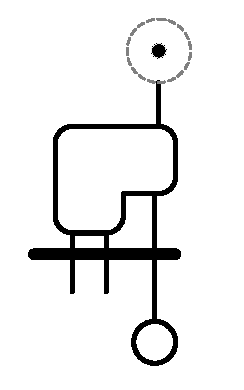
\includegraphics[width=.2\textwidth]{figures/Squiggle.pdf}
\end{center}  


% \vspace{2em}
\vspace*{\fill}

\noindent
\textsf{Last Compiled: \today}

\noindent
\textsf{Image: Birdtrack notation for tensor contraction}

\noindent
\textsf{CC BY-NC-SA 4.0}~\ccbyncsa 

\noindent % Course notes URL
% \url{https://github.com/fliptanedo/P231-2023-Math-Methods}

%% Front page logos
\vspace*{\fill}
\begin{center}

\includegraphics[height=.1\textwidth]{figures/FlipAmbigram.png}
\hspace{5em}

\includegraphics[height=.1\textwidth]{figures/UCRPnA_banner.png}
\end{center}

\newpage

\small
\setcounter{tocdepth}{2}
\tableofcontents
\normalsize
\clearpage
\restoregeometry        %% Return to lecture note geometry 
\pagenumbering{arabic}  %% Turn on regular page numbers


%%%%%%%%%%%%%%%%%%%%%
%%%  THE CONTENT  %%%
%%%%%%%%%%%%%%%%%%%%%

%% TEMPLATE STUFF
% %!TEX root = lecturenotes.tex
%% Update the above with the appropriate root

\chapter{Margins and Figures} %% if using report class

The main difference between my lecture notes and my paper template is the large margin to make use of side notes. The margin is a natural place to encourage students to jot notes and to host useful marginalia.%
\begin{marginfigure}%[th]
    \includegraphics[width=.8\textwidth]{example-image-golden}
    \captionsetup{font={scriptsize,sf}}
    \caption{Example of a margin figure.}
    \label{fig:figure:example:golden}
\end{marginfigure}
You can even place figures in the margin, see Fig.~\ref{fig:figure:example:golden}.\sidenote{Look! No float collision!}

\section{Vision}

This document is inspired by Edward Tufte and the implementation of his ideals in the \texttt{tufte-latex} package. The notes have a large margin for side notes and floats (e.g.\ figures).  Visually this means that the column of main text is narrower, which permits a slightly smaller font.


\section{Using the Margin}

We implement marginalia with the \texttt{sidenotes} package\index{side notes}. We highlight the main usage here. A standard sidenote uses \verb!\sidenote{...}! and looks like this\sidenote{Test of a sidenote. Let's add some extra text here to demonstrate the following point about non-overlapping notes}. Unlike \verb!marginnote!s, \verb!sidenotes! do not overlap with each other.\sidenote{An example of a sidenote that does not overlap with the previous one.} What more, the sidenotes coexist fine with footnotes.\footnote{Here is a foot note.}.

\paragraph{Figures} You can place entire figure floats in the main text region or in the margin. Fig.~\ref{fig:figure:example:golden} is a good example.

All we did was take \texttt{figure}$\rightarrow$\texttt{marginfigure}. You can do the same thing with \texttt{margintable}. On the other hand, sometimes you want a figure that spans the entire text width. Or, perhaps, you want several figures next to each other for comparison. To do this, we simply use the \texttt{figure*} environment. We demonstrate this in Fig.~\ref{fig:subfigure:example:lec}.
\begin{figure*}%[th]
    \centering
    \begin{subfigure}{0.3\linewidth}
    \centering
        \includegraphics[width=\linewidth]{example-image-a}
        \caption{First subfig}
        \label{fig:subfig:1:lec}
    \end{subfigure}\;%
    \begin{subfigure}{0.3\linewidth}
    \centering
        \includegraphics[width=\linewidth]{example-image-a}
        \caption{Second subfig}
        \label{fig:subfig:2:lec}
    \end{subfigure}\;%
    \begin{subfigure}{0.3\linewidth}
    \centering
        \includegraphics[width=\linewidth]{example-image-a}
        \caption{Third subfig}
        \label{fig:subfig:3:lec}
    \end{subfigure}%
    % \captionsetup{font={footnotesize,sf}}
    \caption{Here's how to spread a figure across the entire page, not just the main text width.}
    \label{fig:subfigure:example:lec}
\end{figure*}


We can place large figures in the main text and then place the figure caption in the margin notes. Compare the subfigure in Fig.~\ref{fig:subfig:3:lec} of Fig.~\ref{fig:subfigure:example:lec} to Fig.~\ref{fig:figure:example:golden:sidecap}.
\begin{figure}%[th]
    % \centering
    \sidecaption[][-2\baselineskip]{%
        Example of a margin figure. Note that the \texttt{label} command must be inside the \texttt{sidecaption}. (See source.)
        %
        %% \label command inside the \sidecaption command
        \label{fig:figure:example:golden:sidecap}
    }
    \includegraphics[width=\textwidth]{example-image-golden}
\end{figure}

\section{Other types of marginalia}

Sometimes you can use \texttt{marginnote} to place a note without a marking.\marginnote{See?} Note that \texttt{marginnote} does not, by default, use the same font as \texttt{sidenote}, so we had to set this in the preamble (\texttt{FlipLectureMacros.tex}).


Maybe we want to put another type of float in the margin?
What about a table, like Table~\ref{tab:margin:Table}?
% 
\begin{margintable}[-1em]
\small
    \begin{tabular}{ @{} llll @{} } \toprule % @{} removes space
        Element 
        & Core
        & Mantle
        % & $C_\text{cap}^N (\text{s}^{-1})$ 
        \\ \hline
        Iron 
        & 0.855 
        & 0.0626 
        % & $9.43\times 10^{7}$ 
        \\
        Nickel 
        & 0.052 
        & 0.00196 
        % & $7.10\times 10^{6}$ 
        \\
        Silicon 
        & 0.06 
        & 0.210 
        % & $2.24\times 10^{6}$ 
        \\
        Magnesium 
        & 0 
        & 0.228 
        % & $1.05\times 10^{6}$ 
        \\ \bottomrule
    \end{tabular}
    \captionsetup{font={scriptsize,sf}}
    \caption{Example of a margin table.}
    \label{tab:margin:Table}
\end{margintable}
One curious thing is that \texttt{margintable} does not float independently like a \texttt{sidenote}. Just be a bit careful using this since sometimes it requires manual spacing.
Another curiosity is that in my setup \texttt{sidefigure} and \texttt{sidetable} from the \texttt{sidenotes} package do not seem to work. I think may be because I played around a bit to try to make the \texttt{sidenote} font uniform.

\section{Breaking the Margin}


We define an environment \texttt{wide}\index{wide} that allows text, like equations, to spill into the margins. For example:
\begin{wide}
\begin{align}
f &= \sin\mleft(\frac{x^2}{2}\mright)
\times \arctan t 
\times \log \mleft(\cos \theta\mright)
\times \int_a^b \D{}x \exp\mleft(a^1 + b^2 + x^2\mright)
\times e^{-i\pi} 
\times \Gamma(n) 
\times _{n\!}\text{C}_m
\end{align}
\end{wide}
\begin{wide}
The definition of the margin spillover in \texttt{wide} needs to be matched to the size of the margin defined with the \texttt{geometry} package. Here's what normal text looks like.  The user must be responsible not to place any sidenotes while inside the \texttt{wide} environment.
\end{wide}


\section{Subsequent side notes}

One reason we use \texttt{sidenotes} instead of \texttt{marginnotes} is that \texttt{sidenotes} treats the notes as floating environments that do not overlap with one another.\sidenote{Here is a side note.} These side notes may cause warnings, but should not overlap.\sidenote{Here is another side note that should not overlap.}

Here's a sentence with some citations.\sidenote{Let's make this work. $\e^{i\pi} = -1$.}



\section{Some common environments}

\begin{theorem}[Euler's Identity]
\label{thm:euler:identity}
    Euler's identity\index{Euler's identity} is
    \begin{align}
        \e^{i\pi} = -1 \ .
    \end{align}
    Note that we use the macro \verb!\e! for an upright $\e$ rather than an italicized $e$.
\end{theorem}

\begin{exercise}
\label{ex:derive:euler:identity}
    Derive Euler's identity, Thm.~\ref{thm:euler:identity}.
\end{exercise}

\noindent Good students\index{good students} do the exercises, like Exercise~\ref{ex:derive:euler:identity}. Good instructors provide lots of examples, like Example~\ref{eg:easy:example}.

\begin{example}
\label{eg:easy:example}
    Consider the geometric series
    \begin{align}
        S = \sum_{n=0} a^n \ .
    \end{align}
    We can find a closed form expression for $S$ using
    \begin{align}
        S - aS &= 1\\
        S &= \frac{1}{1-a} \ .
    \end{align}
\end{example}

\section{Some specialized environments}

\begin{bigidea}[Principle of Easy Examples]
\label{idea:easy:examples}
The examples in a book are typically much simpler than the exercises.\sidenotemark
\end{bigidea}\sidenotetext[][-2.4em]{Don't you hate it when this happens?\label{sidenote:in:environment}}

\noindent  Notice that \bigidearef{}~\ref{idea:easy:examples} has a sidenote. Ordinarily \verb!\sidnote{}! does not work in environments. To hack this manually\sidenote{And only do this sparingly!} one may use \verb!\sidenotemark! inside the environment to place the marking and then 
\begin{quotation}
\verb!\sidenotetext[][-2cm]{sidenote}!
\end{quotation}
to implement the sidenote with a manual vertical adjustment.



\section{References}

We use \texttt{biblatex} (not \BibTeX{}) to place references as footnotes.\sidenote{Unlike \BibTeX{}, biblatex does not have a fancy logo. It is simple to make one up: \BibLaTeX{}.} This is because in pedagogical material, you \emph{want} readers to engage with references. Thus it makes sense to put the reference on the same page that you refer to them rather than sequestered at the end of a chapter or---worse---the end of the document. Here is a test citation using \texttt{autocite}: some paper.\autocite{Feng:2016ijc} What is nice is that \BibLaTeX{} is clever with repeated citations.\autocite{Feng:2016ijc} Notice how it does not dump all of the bibliographic data, just what you need to remember the paper and a hyperlink to the original footnote with the full reference. It even takes \texttt{arXiv} identifies with no additional modification.


% \chapter{Paper examples}

% Here are the standard examples I use for my \texttt{paper} template. I include them here to check that nothing has broken. These do not make use of the margin at all. You can see what happens when some text spills into the margin unintentionally.

% %!TEX root = paper.tex
%% Update the above with the appropriate root

\section{Common environments}

\subsection{Figures: floating and wrapped}

\begin{figure}%[th]
    \centering
    \includegraphics[width=0.4\textwidth]{example-image-a}
    \caption{The figure environment shows up often.}
    \label{fig:figure:example}
\end{figure}


\begin{figure}%[th]
    \centering
	\begin{subfigure}{0.3\textwidth}
    \centering
        \includegraphics[width=\linewidth]{example-image-a}
        \caption{First subfig}
        \label{fig:subfig:1}
    \end{subfigure}\;%
    \begin{subfigure}{0.3\textwidth}
    \centering
        \includegraphics[width=\linewidth]{example-image-a}
        \caption{Second subfig}
        \label{fig:subfig:2}
    \end{subfigure}\;%
    \begin{subfigure}{0.3\textwidth}
    \centering
        \includegraphics[width=\linewidth]{example-image-a}
        \caption{Third subfig}
        \label{fig:subfig:3}
    \end{subfigure}%
    \caption{Here's how to use subfigures}
    \label{fig:subfigure:example}
\end{figure}

Use 
% \textbackslash\texttt{centering}
\verb!\centering!
rather than the \texttt{center} environment in figure environments to avoid adding extra vertical space.\footnote{\url{https://tex.stackexchange.com/a/23653/8094}\label{foot:centering}}

\begin{wrapfigure}{l}{0.3\textwidth}
	\includegraphics[width=0.9\linewidth]{example-image-a}
	\caption{via \texttt{wrapfigure}.}
	\label{fig:wrapfig}
\end{wrapfigure}
\lipsum[1]

\subsection{Figures in Equation Environments}
\label{sec:figs}

\begin{align}
	\vcenter{
		\hbox{\includegraphics[width=.1\textwidth]{{example-image-a}}}
		}
	&=
	i g \gamma^\mu \ . 
	\label{eq:vector}
	\\
	\vcenter{
		\hbox{\includegraphics[width=.1\textwidth]{{example-image-a}}}
		}
	&=
	g \gamma^\mu\gamma^5 \ . 
	\label{eq:axial}
	\\
	\vcenter{
		\hbox{\includegraphics[width=.1\textwidth]{{example-image-a}}}
		}
	&=
	ig  \ . 
	\label{eq:scalar}
	\\
	\vcenter{
		\hbox{\includegraphics[width=.1\textwidth]{{example-image-a}}}
		}
	&=
	g \gamma^5 \ . 
	\label{eq:pseudo}
\end{align}


\subsection{Best practices for tables}
\label{sec:tables}

% \begin{table}
	% \renewcommand{\arraystretch}{1.3} % spacing between rows
	% \centering
	\begin{tabular}{ @{} llll @{} } \toprule % @{} removes space
		Element 
		& Core MF 
		& Mantle MF 
		& $C_\text{cap}^N (\text{s}^{-1})$ 
		\\ \hline
		Iron 
		& 0.855 
		& 0.0626 
		& $9.43\times 10^{7}$ 
		\\
		Nickel 
		& 0.052 
		& 0.00196 
		& $7.10\times 10^{6}$ 
		\\
		Silicon 
		& 0.06 
		& 0.210 
		& $2.24\times 10^{6}$ 
		\\
		Magnesium 
		& 0 
		& 0.228 
		& $1.05\times 10^{6}$ 
		\\ \bottomrule
	\end{tabular}
	% \caption{
		% Mass fractions of the Earth's core and mantle.
		% \label{table:elements}
% 	}
% \end{table}




\section{Labels and cleveref}
\label{sec:labels:and:cleveref}

\subsection{\texorpdfstring{\texttt{cleveref}}{cleveref}}
\label{sec:cleveref}

\texttt{cleveref} is a handy package when referring to ranges of equations. 

The pseudoscalar rule is:
\begin{itemize}
	\item Using \texttt{amsmath.sty}'s \texttt{eqref}: \eqref{eq:pseudo}
	\item Using \texttt{cleverefs}'s \texttt{cref}: \cref{eq:pseudo}
\end{itemize}

The equations above are
\begin{itemize}
	\item Using \texttt{amsmath.sty}'s \texttt{eqref}: \eqref{eq:vector} -- \eqref{eq:pseudo}
	\item Using \texttt{cleverefs}'s \texttt{crefrange}: \crefrange{eq:vector}{eq:pseudo}
\end{itemize}

The equations above are (glomped together)
\begin{itemize}
	\item Using \texttt{amsmath.sty}'s \texttt{eqref}: \eqref{eq:vector}, \eqref{eq:axial}, \eqref{eq:scalar}, \eqref{eq:pseudo}
	\item Using \texttt{cleverefs}'s \texttt{cref}: \cref{eq:vector,eq:pseudo,eq:axial,eq:scalar}
\end{itemize}

\texttt{cleveref} automatically identifies the type of object it is referring to. Thus you can use \verb!\cref! to refer to any label, for example \cref{foot:centering}. You can use \verb!\Cref! to have a capitalized the cross reference name. For example: the sections above are \Cref{sec:macros,sec:cleveref,sec:figs,sec:tables}.


\subsection{Sub-equations}

One can also wrap a \texttt{align} environment with a \texttt{subequations} environment. The \texttt{subequations} environment can be given a label. For example,
\begin{subequations}\label{eq:subequations}
\begin{align}
	a &= \pi 
	\label{eq:subequation:1}
	\\
	b &= \e^{\I \pi} 
	\ .
	\label{eq:subequation:2}
\end{align}
\end{subequations}
where we can now refer to the pair of equations \eqref{eq:subequations} or simply one of the equations, \eqref{eq:subequation:2}. This also works in \texttt{cleveref}: \cref{eq:subequations} and \cref{eq:subequation:2}.


\subsection{Referring to Equations}

One style suggestion is to use parentheses to refer to an equation with no additional modifiers \emph{except} at the beginning of a sentence.\footnote{\url{https://academia.stackexchange.com/a/21793}} For example: ``The second term in (3)...'' and ``Equation~(3) has two terms...''



\section{Macros}
\label{sec:macros}


\subsection{Modest capitalization}

Small caps are useful when your text contains acronyms and you do not want them to visually imply emphasis. In other words, we can use them as `not shouting' capitalization. We define a macro \texttt{acro} for this purpose. The default is for \texttt{acro} to be a wrapper for \texttt{small}. Here is an example:
\begin{itemize}
	\item \acro{AdS} in \acro{5D} at the \acro{LHC}.
	\item AdS in 5D at the LHC. 
	\item A third list item to test list spacing.
\end{itemize}


\subsection{Macros for Collaboration}

There are many ways to add notes when collaborating on a document. I like in-line notes with an author name and a color.  \flip{This is an example of a comment.} It is also useful to have a macro for highlighting new text and for proposing the removal of old text.\footnote{Git does this automatically at the level of source code. \texttt{LaTeXDiff} ostensibly does this automatically, but is prone to compile errors and is notoriously difficult to troubleshoot.}

\new{
I fixed the equation:
\begin{align}
	a=b^2 
	\label{eq:samename}
\end{align}
It has label \texttt{eq:samename}. 
}

\remove{
	% It is good practice to indent the `to-be deleted' text
	Here is an equation:
	\begin{align}
	a=b 
	\label{eq:samename}
	\end{align}
	It has label \texttt{eq:samename}.
}

This is essentially a manual version of the \texttt{latexdiff} command. This command can be notoriously fussy around math environments. I personally advocate for using \texttt{git}-related tools to quickly identifying where a version was edited and then using tags to identify edits that need to be highlighted for further discussion. One nice thing about the \texttt{remove} tag above is that it also strips any \texttt{label}s so that there are no `multiply defined label' warnings and one can uniquely refer to a single equation, \eqref{eq:samename}.

\begin{flipcomment}
This is an extended comment that shows up as a text box. I might use this to make some ponderous point about why I think my version of a draft paragraph is more appropriate than yours.
\end{flipcomment}


\subsection{\texorpdfstring{\texttt{xspace}}{xspace}}

The \verb!\xspace! command is useful at the end of a macro. It stands for: ``insert a space if and only if there is supposed to be a space.'' Consider the following examples:
\begin{itemize}
	\item Without \texttt{xspace}: \LaTeX typesetting...
	\item With \texttt{xspace}: \LaTeX\xspace typesetting...
	\item Without \texttt{xspace}: Typeset with \LaTeX.
	\item With \texttt{xspace}: Typeset with \LaTeX\xspace.
\end{itemize}
However, one should consider \verb!\xspace! depreciated. It can be useful for spacing with user-defined macros. However, the results can be unreliable.\footnote{\url{https://tex.stackexchange.com/a/86620/8094}}  For example, one could define \verb!\newcommand{\test}{{test}\xspace}!, note the extra pair of braces in the definition. Even though there is an \verb!\xspace!, this command will fail to place a space between \verb!\test \test!. This type of problem shows up for me because I have a macro \verb!\acro{}! for making acronyms smaller. If I define a shortcut \verb!\newcommand{\DM}{\acro{DM}}! then there is no space between \verb!\DM \test!. The result is: \acro{DM}\xspace {test}. 

The suggested practice is to end your commands with empty braces or a slash: \verb!\DM{}! or \verb!\DM\!. All spacing works out as intended. 
\begin{itemize}
	\item \verb!\DM{} Halo! produces \DM{} Halo
	\item \verb!\LaTeX Fails.! produces \LaTeX Fails.
	\item \verb!\LaTeX{} Works.! produces \LaTeX{} Works.
\end{itemize}






\section{Mathematics and Physics}

\subsection{Environments}

Use the \texttt{align} environment instead of \texttt{eqnarray}, see the TeXblog discussion\footnote{\url{https://texblog.net/latex-archive/maths/eqnarray-align-environment/}}. The double dollar sign notation for \texttt{displaymath} is depreciated.\footnote{\url{https://tex.stackexchange.com/questions/503/why-is-preferable-to}} The suggested alternative is \verb!\[! and \verb!\]!, though this is rather annoying. As a default I always use \texttt{align}.

Single dollar sign \verb!$! notation is also depreciated relative to \verb!\(! and \verb!\)! for inline text. However, I am stubborn about keeping in-line text as simple as possible. The dollar sign is a single character and it is visually easier to identify as a delimiter for math mode. I thus continue using single dollar signs for inline mathematics. 


\subsection{Text and Math: super- and subscripts}

Use the \texttt{text} command to insert text into math environments. For subscripts use \texttt{textnormal}. 
% 
We use the \texttt{textnormal} command for super- or subscripts rather than the \texttt{text} command because this automatically uses the correct size. Compare, for example: $G_\textnormal{D},\, G_\text{D}$.

One place this shows up is if you have a subscript that is not a mathematical variable. For example, $x_a$ makes sense for the value of $x$ at point $a$, but $x_\text{b}$ should be used if the `b' is shorthand for boundary. Similarly, $E_\text{max}$ for the maximum energy, rather than $E_{max}$.


\subsection{Units and spacing}

Use a tie (tilde) to enforce a non-breaking short space between a number and its units: $0.5~\text{MeV}$. Units should not be italicized. If you want to be svelte you can use a thin space, \verb!\,!. Some people like the \texttt{siunitx} package; I find it a little cumbersome for that it is, especially given that I usually write in natural units.

Some care is required for spacing with math operators\footnote{\url{https://tex.stackexchange.com/a/35585/8094}}. Here's a guideline for how to use different bits of manual spacing\footnote{\url{https://tex.stackexchange.com/questions/25810/when-one-should-use-spacing-line-quad-or}}.


\subsection{Upright characters}

These come from the \acro{ISO 80000} standards for typesetting mathematics and physics.\footnote{See discussion in \url{https://tex.stackexchange.com/q/14821/8094}} It is not obvious to me that these are applicable to the typographical culture of physics, but the most important thing is to be consistent.
\begin{itemize}
	\item Units are always upright, \textmu m is a micrometer. You can use various unit packages to do this automatically. 
	\item The base of the natural logarithm is upright $\e^{i\pi}$ versus $e^{i\pi}$. The best physics argument is to avoid confusion between the exponential $\e$ and the electric coupling $\alpha = e^2/4\pi$.\footnote{I thank Matt Reece for pointing this out to me.}
	\item The differential is an operator so it should be upright. I have macros for this: $dx$ vs.~$\D{x}$ and $\dbar p$ vs.~$\Dbar{p}$. The \texttt{physics} package has macros for this. 
	\item You could also do this for the imaginary number: $a+\I b = \e^{\I \theta}$. This one is a little trickier to get the spacing right. We use \verb!\newcommand{\I}{\operatorname{i}\mkern-2mu}!.
	\item You can use \verb!\DeclareMathOperator! to define upright Roman letters that should be treated as a single operator like $\sin$. This also automatically fixes the spacing after the operator contextually depending on whether the next character is understood as an argument, $\sin x$, or a group $\sin(ax)$.
\end{itemize}
There is a historical discussion on \texttt{hsm.stackexchange}\footnote{\url{https://hsm.stackexchange.com/questions/6727/fracdydx-versus-frac-mathrm-dy-mathrm-dx}}.  For all of these, it helps to define macros. This makes it easy to change the style when you have a co-author who strongly disagrees.

\subsection{Absolute Values}

We define a macro \verb!\abs{}! to invoke \texttt{amsmath}'s \verb!\lvert! and \verb!\rvert! commands for automatically sizing the left- and right-bars of an absolute value. Examples:
\begin{align}
	\abs{x} &&
	\abs{\frac{x}{y}} &&
	\abs{\int \D{x} \, e^{i px}} &&
	\int \D{x} \, \abs{e^{i px}}
	\ .
\end{align}
If you want to be fancier, you can use \texttt{mathtools}\footnote{\url{https://tex.stackexchange.com/a/35585/8094}} to define custom delimiters. For example:
\verb!\DeclarePairedDelimiter{\abs}{|}{|}! \, .


\subsection{Miscellaneous}

\begin{itemize}
	\item Use $\mid$ instead of pipe for conditions: $p(x\mid y)$ versus $p(x|y)$.
	% 
	\item Transpose: The \acro{ISO}~80000 standard has suggestions. $A^T$ vs $A^\top$ vs $A^{\trans}$. I personally prefer $A^\text{T}$.
	% 
	\item \textbf{Textual subscripts}: sometimes you have a subscript that is not an index, but shorthand for something textual. For example, the Green's function with Dirichlet boundary conditions is $G_\textnormal{D}$. The subscript is upright, not italicized, $G_D$. Use the \texttt{textnormal} command rather than the \texttt{text} command since this will automatically use the correct size. Comparison: $G_\textnormal{D},\, G_\text{D}$.
	% 
	\item Arrows with text under them: \texttt{xrightarrow} in the \texttt{amsmath} package. The square bracketed argument is under, the curly bracketed argument is over. Example: $\xrightarrow[\textnormal{low}]{\textnormal{hi}}$.
	% 
	\item We can use the $\defeq$ symbol, defined as a macro\footnote{\url{https://tex.stackexchange.com/a/4881/8094}} \verb!\defeq!, to denote assignment . The macro typesets the symbol so that the dots are the same size and aligned with the lines. In pedagogical writing, it may be useful to distinguish between equality $=$, assignment $\defeq$, and tautology $\equiv$. At least that is how I use these.\footnote{Arnold Arons brings up equal signs in \emph{Teaching Introductory Physics}, Chapter~3.23. I prefer $\defeq$ for definitions because it shows the asymmetry of the relation. The statement $a\defeq b$ means that $a$ is defined to be $b$. The equal sign $=$ is symmetric in appearance and in meaning: $a$ and $b$ are the same. I use  $a\equiv b$ sparingly to mean $a$ and $b$ are \emph{obviously} the same but in a way that is not necessarily derived mathematically. }
\end{itemize}



\section{Space}

\subsection{Kerning: spacing between characters}
Math operators have a natural spacing before and after depending on the context. In the following example, spaces indicate that the coefficient $a$ multiplies the logarithm of $b$:
\begin{align}
	a\log b && a\log(bc)
\end{align}
The space on either side of $\log$ indicate that $\log$ is a mathematical operator. The second example still has the space between $a$ and $\log$, but has no space between $\log$ and $(bc)$ because the parenthesis belongs to the mathematical function.\footnote{Example from \url{https://tex.stackexchange.com/a/140647}}
% 
You can use \verb!\DeclareMathOperator! for functions that are not built in.

Using \verb!\left(! and \verb!\right)! will automatically size parentheses, but can mess up kerning:
\begin{align}
	f(x)
	f\left(x\right)
	f{\left(x\right)}
	&
	&
	\cos(x)
	\cos\left(x\right)
	\cos{\left(x\right)}
	{\cos}{\left(x\right)}
	\ .
\end{align}
The crude way to fix this is to put braces around the parentheses: \verb!{\left(x\right)}!.\footnote{\url{https://tex.stackexchange.com/a/2610/8094}}. However, if the parenthesis is attached to a mathematical operators, the operator must also be surrounded by braces: \verb!{\cos}!. In the examples above, you can see the effect of the braces on the spacing on either side.



\subsection{Manual Spacing}

\LaTeX{} has commands for manually inserting spacing: 
\begin{itemize}
	\item \verb!\,! thin\,space
	\item \verb!\:! medium\:space
	\item \verb!\;! thick\;space
	\item \verb$\!$ thin\!negative\!space.
		  %% note the use of a different symbol in \verb 		
\end{itemize}
The negative space can be helpful for manually adjusting the kerning for large parentheses raised to a power:
\begin{align}
	\left(\frac{\pi}{\sum_{i=1}^n x^i}\right)^{d+1}
	&&
	\left(\frac{\pi}{\sum_{i=1}^n x^i}\right)^{\!d+1}
	\ .
\end{align}
On the right we use \verb$\right)^{\!d+1}$.



\subsection{Ties create non-breaking spaces}

\LaTeX{} interprets periods as full stops (end of a sentence). It places extra space after the full stop. Use a \textbf{normal space} right after the period, \verb!.\ ! (``slash space'') to tell \LaTeX{} that a period is not a full stop and that it should insert insert a normal space not a double space.\footnote{The double space is sometimes considered old fashioned. You can use \texttt{frenchspacing} in your document to turn off the double space after a full stop.} Mr.\ Roboto versus Mr. Roboto. 


% Use a \textbf{tie} (tilde) when a period is not a full stop: Mr.~Roboto versus Mr. Roboto. 
A related construction is a \textbf{tie} (tilde). This gives \textbf{non-breaking space} which is a normal space that \LaTeX{} interprets as `part of the word'. This means that line breaks should not occur along the non-breaking space.
% 
You can also use ties this whenever you want to prevent a line break between words. \LaTeX{} interprets the tied words as a single word.
% 
Ties are also standard for citations: \verb!Tanedo et al.~\cite{citation}!. 




\section{Some Best Practices}

\subsection{\texorpdfstring{\LaTeX{} in a title}{LaTeX in a title}}

When using \LaTeX{} code in a section title, use the \texttt{texorpdfstring} command to define an \acro{UTF-8} string that the pdf can use for bookmarks. If you do not do this, there are annoying compilation warnings.


\subsection{Ranges}

Hyphens, en dashes, em dashes, and minus signs in math mode are all grammatically different.
\begin{itemize}
	\item En dashes replace hyphens in a compound adjective where one of the elements is a two-word compound: `post--Cold War era.'\footnote{From \url{https://www.merriam-webster.com/words-at-play/em-dash-en-dash-how-to-use}}
	\item En dashes are used for combinations of two names in place of the word `and.' For example, Randall--Sundrum model.
	\item For compound names of a single person, use a hyphen: Levi-Civita.
	\item A minus sign should be typeset in math mode, $-1$.
\end{itemize}
The choice between a hyphen and en dash can be tricky. For example \acro{APS} seems to prefer ``anti--de Sitter'' with an en dash, whereas others prefer a hyphen.\footnote{See 1 Jan '23: \url{https://en.wikipedia.org/wiki/Talk:Anti-de_Sitter_space}.}


\subsection{References}

Use \BibTeX\xspace. There are any number of \BibTeX\xspace managers. One that I like is Yuji Tachikawa's \texttt{spires.app}\footnote{\url{https://member.ipmu.jp/yuji.tachikawa/spires/}}; it links directly to the inSpire \acro{HEP} database. For styling, I recommend Jacques Distler's \texttt{utcaps.bst} which is a nice format that automatically inserts a hyper link to the \texttt{arXiv} version of a paper. If yo are fancy you may use {\rm B\kern-.05em{\sc i\kern-.025em b}\LaTeX{}. 


Standard citation managers with \BibTeX\xspace capability make a big deal about assigning unique \BibTeX\xspace citation keys to each reference. This can be tedious if you have to collaborate with someone else who has made up their own citation keys. Fortunately, in my field there is a single recognized database, inSpire\footnote{\url{https://inspirehep.net}; see also \acro{NASA/ADS} for astronomy.}, that assigns a unique \BibTeX entry for papers.  This means that it is good practice to select keys as follows:
\begin{itemize}
	\item If it exists, use the inSpire key. Tools like \texttt{spires.app} default to this key.
	\item If inSpire does not have the reference, use \acro{NASA/ADS}.
	\item If neither of those databases has the references, find a simple algorithm that all of your coauthors can agree upon. 
\end{itemize}
Items in the third category are usually books and websites. 



\section{Neat examples}

Suppose you would like to repeat and equation reference,
\begin{align}
	\e^{\I\pi} &= -1 
	\ .
	\label{eq:e:ipi}
\end{align}
Remember that equation above? Let's write it again,
\begin{align}
	\e^{\I\pi} &= -1 
	\ .
	\tag{\ref{eq:e:ipi}}
\end{align}
Observe that these have the same equation number. Instead of \texttt{label} we use \texttt{tag} with argument \texttt{ref}.

% %!TEX root = paper.tex
%% Update the above with the appropriate root

\section{Teaching Examples}

For lecture notes it is useful to have some framed environments to highlight examples and exercises. In the past I have used \texttt{framed} and \texttt{mdframed}. I think \texttt{tcolorbox} may be the best option now.

% \begin{tcolorbox}
% 	⟨environment content⟩
% \end{tcolorbox}

\begin{theorem}[Flip's Theorem]
This is an example theorem.
\end{theorem}

\begin{example}[Flip's Example]
This is an example of an example
\end{example}


\begin{exercise}[Solving a differential equation]
  Solve the following differential equation.
  \label{ex:solve:ode}
\end{exercise} 
\noindent Can you solve Exercise~\ref{ex:solve:ode}?


\begin{bigidea}[environments]
  With \texttt{tcolorbox}, one may `dress' existing environments in boxes. The call to the environments is unchanged.
  \label{idea:environments}
\end{bigidea} 
\noindent Refer to \bigidearef{}~\ref{idea:environments}.
% %!TEX root = paper.tex
%% Update the above with the appropriate root

\section{Code example}

These are examples of the \texttt{listings} package for typesetting code. See Overleaf\footnote{\url{https://www.overleaf.com/learn/latex/Code_listing}} and \acro{TeX.SE}~\footnote{\url{https://tex.stackexchange.com/a/350242}} for more information. By the way, printed out code is called `listings' because old computer languages has a \texttt{LIST} command to print out the numbered source code lines.\footnote{\url{https://softwareengineering.stackexchange.com/a/289729}}

\subsection{Inline}

If you just want to be able to insert \LaTeX{} into a document like this, you can use \verb!\verb!\footnote{\url{https://stackoverflow.com/a/66115768/16426341}}. The way it works is that you write \verb!\verb#TEXT#! where \verb!#! is any character that is not in \texttt{TEXT}. You can use listings package similarly with \verb!\lstinline! in place of \verb!\verb!.


\subsection{Jupyter Notebook}

Jupyter formatting from user \texttt{yogabonito} on \acro{TeX.SE}\footnote{\url{https://tex.stackexchange.com/a/350242/8094}}.

\begin{pyin}%[pyin01]
print("Hello world")
\end{pyin}
%  
\begin{pyprint}
Hello world
\end{pyprint}
% 
You get a `multiply defined label' warning if you do not explicitly label each of your Python inputs. 
%% EXAMPLE: 
% \begin{pyin}
% print("Hello world, too")
% \end{pyin}
% \begin{pyin}
% print("Hello world, three.")
% \end{pyin}
%% This gives two Python inputs with label `' (blank)
%% and thus returns a compiler warning.
% 
% 
Here we have a return value in the last line of the input cell.
\begin{pyin}[labelOfTheSecondInput]
def twicify(arg):
    print("Received:", arg, "- Will double now...")
    return 2 * arg
twicify(1)
\end{pyin}

\begin{pyprint}
Received: 1 - Will double now...
\end{pyprint}

\begin{pyout}
2
\end{pyout}
% 
% \subsection{Referencing input}
You can also reference the labeled input \ref{labelOfTheSecondInput}, from above.
% \begin{pyin}[anotherlabel]
% "and the counter will automatically do the right thing :)"
% \end{pyin}
% \begin{pyout}
% 'and the counter will automatically do the right thing :)'
% \end{pyout}


\subsection{\texorpdfstring{\LaTeX}{LaTeX}}

From user \texttt{hair-splitter} on \acro{TeX.SE}\footnote{\url{https://tex.stackexchange.com/a/637305/8094}}:

\begin{lstlisting}[style=latexstyle]
\documentclass{article}
\usepackage[T1]{fontenc}
\newcommand*{\mycommand}{Hello World!}
\begin{document}
  \mycommand
\end{document}
\end{lstlisting}


% %!TEX root = paper.tex
%% Update the above with the appropriate root

\section{\texorpdfstring{\LaTeX{} Style}{LaTeX Style}}

There is not a definitive \LaTeX{} style guide analogous to \acro{PEP-8}. However, I do have my own set of preferences. Here style refers to how the \LaTeX{} source files are written. Two \texttt{tex} files may produce identical \texttt{pdf} outputs but be stylistically different. A well styled document is that is as easy as possible to parse and edit as a human being. I have done my best to keep the source files for \emph{this} template well styled.


\subsection{Idiosyncracies}

While some coding style guides require a fixed width for the document. This gives meaning to a line of code and makes the resulting source more readable by avoiding unintentional text wrapping. \LaTeX{} is a bit different in that it is a typesetting language that is meant to handle paragraphs of text. Because modern editors naturally have text wrapping options, I do not feel strongly about enforcing a document-wide character width limit. Paragraphs of text should be allowed to wrap if that makes sense. However, mathematics environments should strive to make use of white space in service to readability.


\subsection{Spacing and Indents}

White space helps distinguish the document structure. 

\begin{enumerate}
	\item Sections should have three empty lines between each other.
	\item Sub-sections should have two empty lines between each other.
	\item All other units of paragraphs should have one empty line space between them.
\end{enumerate}
One may use with commented out empty lines to separate sentences from one another. 
% 
	This produces no paragraph break between the sentences in the output, but can help separate different ideas within a paragraph.
% 
	Similarly, one can combine this with indents to help visually organize the logical flow of a paragraph.


\subsection{Mathematics}

Use comments and white space to separate mathematics environments from plain text.
% 
The contents of a mathematics environment should use ample white space to separate each mathematical object as if these were words in a sentence.
% 
\begin{lstlisting}[style=latexstyle]
\begin{align}
  S_{\textnormal{fix}}^{\textnormal{Bulk}}
  & =
  \frac{-1}{g^2} 
  % \int d^{d+1} x  
  \int \DD{d+1}{x}
  \left( \frac{R}{z} \right)^{\!d-3}
  \frac{1}{2\xi}
  \left[
    \partial_\mu A^\mu
    -
    \xi\left( 
      z^{d-3} 
      \partial_z \left( \frac{A_z}{z^{d-3}} \right)
      -
      \left( \frac{R}{z} \right)^{\!2} 
      g^2 v(z) \, \pi
    \right)
  \right]^2 \ ,
\label{eq:SGFBulk}
\end{align}
\end{lstlisting}
% 
This produces the following:
\begin{align}
	S_{\textnormal{fix}}^{\textnormal{Bulk}}
	& =
	\frac{-1}{g^2} 
	% \int d^{d+1} x  
	\int \DD{d+1}{x}  
	\left( \frac{R}{z} \right)^{\!d-3}\frac{1}{2\xi}
	\left[
	    \partial_\mu A^\mu
	    -
	    \xi\left( 
	        z^{d-3} \partial_z \left(\frac{A_z}{z^{d-3}}\right)
	        -
	        \left(\frac{R}{z}\right)^{\!2} g^2 v(z)\, \pi
	    \right)
	\right]^2 \ ,
% \label{eq:SGFBulk}
\end{align}
For long expressions, each line should be a well-defined `unit' of the mathematical expression. When there are multiple `words' in an expression, add white space to delimit them. The use of indentation to group elements of the same level should be self explanatory.

For example, simple fractions do not need any white space, while more complicated fractions should provide some help:
% 
\begin{lstlisting}[style=latexstyle]
\frac{ 
	b_\mathcal{O}
}{
	\Lambda^{\Delta_\mathcal{O} - \frac{d}{2} - 1 }
} 
\end{lstlisting}
% 
This may seem like overkill, but in an expression with multiple fractions it is helpful to be able to quickly visually parse each piece of the expression.


\subsection{When (not) to use macros}

Use macros (\texttt{newcommand} or \texttt{renewcommand}) when there is an expression that you use often \emph{and that you may want to change in the future}. Perhaps you have a variable that needs to be used uniformly across a document, but whose specific symbol may change. Use a macro and make it easy to change that symbol without doing a find-and-replace. Macros are also useful for making \LaTeX{} source more readable by truncating a tedious series of commands. 

However, do not use a macro just because it will make your life easier in the moment. One good reason \emph{not} to use a macro is as a shortcut for defining an environment. There is a `old style' of source preparation where someone will define macros:
% 
\begin{lstlisting}[style=latexstyle]
\newcommand{\be}{\begin{equation}}
\newcommand{\ee}{\end{equation}}
\end{lstlisting}
% 
This seems like a shortcut because it saves you the trouble of writing
% 
\begin{lstlisting}[style=latexstyle]
\begin{equation}
	...
\end{equation}
\end{lstlisting}
% 
There is a narrow range of tech-savvy for which this `trick' is useful: one has to be sophisticated enough where typing in six characters rather than thirty-one characters will save significant time, but one must also be na\"ive enough to not use a text editor that can do (1) text expansions or (2) context-aware text highlighting. 
% 
This latter point is what can drive a collaborator crazy: some \LaTeX{} editors look for \textbackslash\texttt{begin}--\textbackslash\texttt{end} pairs to identify math mode and highlight text in a helpful way. Macros like \texttt{be} and \texttt{ee} screw this up and can lead to linter warnings. In summary, do not define macros to simplify environments.


\subsection{Labels}

Labels should be descriptive, even if that means that they labels become a bit lengthy. Each label should start with some indication of what it is labeling, \texttt{eq} for equation or \texttt{fig} for figure, for example. Use colons to separate words.
% 
\begin{lstlisting}[style=latexstyle]
\label{eq:Euler:formula}
\label{sec:introduction}
\label{sec:introduction:past:work}
\end{lstlisting}
% 
Many \LaTeX{} editors have intelligent autocomplete that makes it easy to insert references to past labels, so it does not take any more time to have a lengthy label. It does, however, save time if your labels are descriptive and easy to select from a drop-down menu. 


\subsection{Collaborative writing}

A key principle of \LaTeX{} source should be making the document collaboration-friendly. It is \emph{not} sufficient that your \LaTeX{} source compiles. Your code needs to be:
\begin{enumerate}
	\item \textbf{Readable}. Use white space in a consistent way to reflect the underlying structure of your document and your expressions. Use consistent spacing between sections and subsections. Use ample white space within an equation to make each piece easy to identify. 
	\item \textbf{Editable}. Collaborators should be able to fix typos without having to do a deep dive of your source ode. 
\end{enumerate}
Here's what you are allowed to sacrifice in order to meet these goals:
\begin{enumerate}
	\item Your source code does not need to be short. Nobody will print out our source file. An equation that typesets to a single line can be spread out over a dozen lines if it helps the reader parse the \LaTeX{}. 
	\item Your source code does not need to be confined to a single file. 
	\item Your figures should be in a separate folder. In this template we use:
% 
\begin{lstlisting}[style=latexstyle]
\graphicspath{{figures/}}
\end{lstlisting}
% 
	\item Your pose writing---that is, writing that is not in math mode---can also be broken up using empty lines (comment out the line to avoid starting a new paragraph) and white space in order to elucidate the structure.\footnote{This can be useful if you tend to write convoluted sentences. You can `diagram' your sentence so that you see how each clause fits together.}
\end{enumerate}

A good way to collaborate is to use \texttt{git}/\texttt{github} or {Overleaf}. Overleaf is fantastic for abstracting away all version control. However, savvy users with an Overleaf membership can connect to Overleaf documents using \texttt{git}. This gives you the best of both worlds: you may use your favorite \acro{IDE} or \LaTeX{} editor and your favorite \texttt{git} client to synchronize to an Overleaf document that your collaborators can edit through the web interface if they wish.\footnote{You may notice that there is a \texttt{gitignore.txt} file in this template. It is a copy of the \texttt{.gitignore} file used by \texttt{git}. The \acro{macOS} interface does not like it when users try to manipulate files named dot-something since it worries that you might be messing up an important system file. Thus I have included a text file with the contents of \texttt{.gitignore} for users who simply want to copy this template folder using \acro{macOS}. You should then rename \texttt{gitignore.txt} to \texttt{.gitignore} if you are using \texttt{git}. Alternatively, download this file as a template from \texttt{github} and ignore \texttt{gitignore.txt} altogether.  }

\subsection{\texorpdfstring{\LaTeX{} Style Guide}{LaTeX Style Guide}}

\begin{itemize}
	\item Use \texttt{hyperref}. Modern documents should be internally and externally hyperlinked. Clicking on a reference to an equation should bring the reader to that equation. Use a bibliography style that allows hyperlinks to the \texttt{arXiv}.
	\item In \emph{informal} documents like this, I refer to websites (usually Stack Exchange) with a footnote and a hyperlink:
	% 
\begin{lstlisting}[style=latexstyle]
...a great website.%
\footnote{\url{https://www...}}
\end{lstlisting}
	% 
	This avoids having to use \BibTeX for one-off references and makes the reference easily clickable. 
	% 
\end{itemize}


\subsection{Copy Editing Style Guide}

These are non-specific style points:

\begin{itemize}
	\item Footnotes go after punctuation.%
			\footnote{Like this.}
	\item Use whitespace to separate footnotes:
	% 
\begin{lstlisting}[style=latexstyle]
We now make an important%
  \footnote{
	Observe the comment and whitespace.
	There is no additional spacing between
	`important' and this footnote. }
point about style.
\end{lstlisting}
	%
	\item You may consider using \textbackslash\texttt{frenchspacing} in your document.\footnote{Hat tip to Eddie Kohler, \url{https://www.read.seas.harvard.edu/~kohler/latex.html}}
\end{itemize}


\subsection{Breaking the rules}

It is okay to break the style rules when doing so supports clarity. Sometimes it makes sense to throw in lots of extra white space to separate ideas.


\subsection{Cleaning Up}

Sometimes it is okay to leave a mess. You may want to preserve an old `verbose' version of your source files that has intermediate steps spelled out overly-pedagogically. You may find it useful to leave comments in the source files to remind yourself of the structure of your argument. These changes are preserved if you use version control, but sometimes you want the redundancy and convenience of having old text readily available. Just remember to go through your source code carefully to strip it of comments before submitting to a public repository like the \texttt{arXiv}.
% %!TEX root = paper.tex
%% Update the above with the appropriate root

\section{References}

\subsection{\texorpdfstring{\LaTeX{} Style}{LaTeX Style}}

\begin{itemize}
    \item Didier Verna, ``Towards \LaTeX{} coding standards.\footnote{\url{https://tug.org/TUGboat/tb32-3/tb102verna.pdf}; video: \url{http://zeeba.tv/toward-latex-coding-standards/}}'' 
    \item See also Philippe Beliveau's summary of Verna's piece.\footnote{\url{https://medium.com/@pbeliveau/latex-coding-standards-f82743b7866b}}
    \item Evan Chen, ``Evan's \LaTeX{} Style Guide.\footnote{\url{https://web.evanchen.cc/latex-style-guide.html}}''
    \item Eddie Kohler, ``LaTeX Usage Notes.\footnote{\url{https://www.read.seas.harvard.edu/~kohler/latex.html}}''
\end{itemize}


\subsection{Style Guides}

Most publications have a style guide, analogous to the well-known \acro{APA} style in social sciences. Checking for strict adherence to those guides have historically been the role of copy editors, though the number of published papers continues to grow with no obvious increase in resources for copy editing. 

\begin{itemize}
    \item There is an \acro{ISO} standard for typesetting mathematics and physics. As of 2023 it is \acro{ISO80000}.
    \item Strunk \& White, \emph{The Elements of Style}
    \item The \emph{Review of Modern Physics} style guide. 
\end{itemize}

\subsection{Typography References}

The standard typography reference is Robert Bringhurst's \emph{The Elements of Typographic Style}. 
The following references focus specifically on typography and \LaTeX{}.
\begin{itemize}
    \item Consistent typography on \acro{TeX.SE}\footnote{\url{https://tex.stackexchange.com/questions/29840/consistent-typography}}
    \item List of best practices references on \acro{TeX.SE}\footnote{\url{https://tex.stackexchange.com/questions/577/best-practices-references}}, including the list of obsolete packages and commands in \LaTeX{}~2e\footnote{\url{https://www.ctan.org/tex-archive/info/l2tabu/english/}}
    \item ``The Art of \LaTeX{},'' a list of guidelines from Fan Pu Zeng\footnote{\url{https://fanpu.io/blog/2023/latex-tips/}}
    \item Showcase of beautiful typography in \LaTeX{}\footnote{\url{https://tex.stackexchange.com/q/1319/8094}}
\end{itemize}



% %% CHAPTER SUBAPPENDIX %% if using report class
% \begin{subappendices}
% \section{Subappendix}\label{sec:subappendix:eg}
% This chapter has its own special appendix.
% \end{subappendices}


\chapter{Introduction}

\section{Two powerful questions}
At any time in this course, you should feel comfortable asking either of the following questions:
\begin{enumerate}
    \item Is it obvious that...?
    \item Why is this significant?
\end{enumerate}
The first question is the way to ask for on-the-spot clarification---I will either appreciate that I did not properly explain a subtle point, \emph{or} I will explain the intuition\sidenote{Your sense of mathematical and physical intuition is incredibly valuable. This is one of the key traits that makes a physics training unique.} for why something should be obvious. The second question is a way to remind me that I may have \emph{lost sight of the forest for the trees}: I want this course to \emph{mathematically connect big ideas in physics}. Asking this question is a reminder that making those connections justifies the hard mathematical work we will put into the course.

\section{Exercises and Examples}
I have tried to insert exercises and examples in these notes. There are still far too few for sound pedagogy. If you really, really want to learn something, you \emph{have} to do exercises. Think of the examples as exercises with solutions---though they are not always written this way. Mull over the exercises: ask yourself why the problems are posed the way they are, challenge the statements to find the domain of validity, think of how one may extend those exercises to other applications. The exercises are a far better gauge of you learning than whether or not you have read a section of the notes. If you are confused reading the text in section 10, it is often the case that you should have been doing the exercises since section 5.

\begin{bigidea}[Do your homework]
Instructors feel no deep satisfaction when you turn in your homework. Instead, an assignment is a pledge to the student to give an opportunity for practice with feedback from someone more experienced.
\end{bigidea}

\section{Obvious-ness}
Finally, I want to comment on the word \emph{obvious}. I write this often. It is somewhat dangerous because it can come off as being arrogant: \emph{this is so obvious to me, if you do not understand you must be deficient}. This is never the reason why I use that word. Instead, the word \emph{obvious} serves a very practical purpose. The goal of this class is not just to be able to ``do stuff'' (e.g.~diagonalize a symmetric matrix), but to also build that intuition that comes from a deeper understanding how the mathematics works. In this sense, every time I write the word \emph{obvious} it is a flag: I am saying something that---with the proper perspective---should be self-evident. If it is not self-evident, then you should stop to interrogate why it is not self-evident. Most likely there is something where a change in perspective may (1) make it obvious, and (2) in so doing deepen your understanding of the subject. So when you see the word `obvious,' I want you to do a quick check to confirm whether or not the statement is indeed obvious. If it is not, then welcome the opportunity to learn.\sidenote[][-3em]{There is, of course, the possibility that what I have written is \emph{not} obvious. For example, if I have made a typo... in which case, please let me know.}



\section{Motivation}

Here are three deeply significant equations in physics:\sidenote{If you want to be fancy, you can add Maxwell's equations. If you want to be \emph{really} fancy, you can write these as $dF=0$ and $-*dF = *J$, but that's for a different course.}
\begin{align}
    \vec{F} &= m\vec{a}
    \\
    % R_{\mu\nu} - \frac{1}{2}Rg_{\mu\nu} 
    G_{\mu\nu}
    &= \frac{8\pi G_\text{N}}{c^4} T_{\mu\nu}
    \\
    \hat H |\Psi\rangle 
    &= E |\Psi\rangle \ .
    \label{eq:three:equations}
\end{align}
These are Newton's force law, Einstein's field equations, and the Schr\"odinger equation. They govern classical physics, general relativity, and quantum theory, respectively. 


Each equation looks rather unique: they seem to each be speaking their own mathematical language. Newton's law is written with boldfaced vectorial quantities $\vec{F} = (F_x, F_y, F_z)^\trans$ that should look very familiar to any physics undergraduate. Einstein's equation has these funny $\mu$ and $\nu$ indices on every term---have you seen these before? Do they look intimidating? If you ever want to make your equations look ``technical'' and ``physicsy,'' you should dress them up with indices. The Schr\"odinger equation has no indices, but instead has these funny angle-brackety things... and that $\hat H$ looks suspicious. Where did $H$ get a hat, and what is the content of this equation other than $\hat H = E$?

\emph{Each of these equations turns out to be a ``vectorial'' equation.} Each one is actually shorthand for a number of equations. Newton's equation is shorthand for three equations, one for each component. Einstein's equation is shorthand for 16 equations, one for each combination of the indices $\mu$ and $\nu$ that run over four values\sidenote{The four values are the three directions of space and one direction of time.}. The Schr\"odinger equation is shorthand for an \emph{infinite} number of equations, one for each allowed energy of a quantum system.

The mathematical formalism that unifies these different ideas (and notations) of `vector' is called linear algebra. It may sound humble: after all, ``linear'' systems are \emph{easy}, aren't they? Did we not just spend years of our lives learning fancy things like \emph{calculus} and \emph{differential equations} to deal with functions that are more complicated than \emph{lines}? In some sense, yes: linear algebra is about lines and planes in different numbers of dimensions.\sidenote{On the other hand: a good chunk of the calculus that we do is also implicitly linear. Physicists often Taylor expand and keep only the $\mathcal O(\varepsilon)$ term. Integration boils down to summing trapezoids whose angley-bits are given by the first derivative of a function... the linear component.} However, linear algebra turns out to be far more richer than what you may be used to from high school. 

In this course we will see how the three equations in \eqref{eq:three:equations} are connected by the mathematics of linear algebra. We will dive into the different notation and shamelessly pass between $\vec{v}$, $v^i$, and $\ket{v}$ to describe the same abstract vector. We will connect to the mathematical description of \emph{symmetry} and see how it is an underlying theme in our descriptions of nature. And we will do all of this in a way that will make the instructors of the linear-algebra-for-mathematicians course and linear-algebra-for-engineers course vomit a little in disgust. Consider that one of privileges of being a physicist.



\chapter{The Basics}

\section{Pre-conceptions}

If this were a mathematics course, then we would start by very carefully defining words like \emph{vector} and \emph{matrix}. As a physics student, you already have a working definition of these words. It is probably something like this:
%
\begin{quote}
A vector has a magnitude and a direction. We write a vector as an array of three numbers arranged in a column. A matrix is an array of nine numbers arranged in a $3\times 3$ block. There is a rule for how to apply (multiply) the matrix to the vector to produce a new vector.
\end{quote}

The problem is that you already know too much to learn linear algebra as a mathematics student. You have already seen the tip of the iceberg and so have preconceptions about what vectors are and how they work. You may remember from freshman mechanics that forces are vectors. So are momenta and velocities. You may also recall the idea of a force field---like the electric field---which is actually a whole bunch of vectors: one for each point in space. Examples of matrices are a little more subtle: you may recall that you can represent rotations as matrices. Speaking of rotations, there was another thing that showed up called the moment of inertia \emph{tensor}. It looked like a matrix, but we never called it the ``moment of inertia matrix.'' What the heck is a tensor, anyway?

And so, you see that starting this course like a mathematics course could cause trouble. The mathematics professor would start by defining a vector. That definition will say nothing about magnitudes or directions, and will not even say anything about arrays of numbers. That definition will clash with the hard-earned intuition that you built from your physics education thus far. It will be perplexing, and may make you feel rather unhappy. What do these mathematicians know, anyway? Or maybe its the physics that is wrong, or have we just completely misunderstood everything and we are just now noticing that we are hopelessly lost? We begin to spiral into a black hole of confusion.

\begin{quote}
Fortunately, \emph{this is not a mathematics course.}
\end{quote}

As a consequence, we will not give a rigorous definition of a vector. We start with a familiar definition of vectors and lay out which qualities are general, and which properties are specific. Then we will come to appreciate the approximation that ``\emph{everything is a vector}.'' So let us start with something comfortably familiar, even though it constitutes only the simplest example of a vector.


\section{Real Three-Vectors}

Let us write $\vec{v}$ to be a vector. This is a standard convention for writing a vector. In this course we will use a few different notations for vectors according to convenience. Notation is neither physics nor mathematics, it is simply a shorthand for a physical or mathematical idea. 

% At this point, you may wonder \emph{what is a vector, anyway?} Maybe a vector is a column with three numbers that represent coordinates in three-dimensional space:
In fact, let us focus on a particular type of vector: \textbf{real three vectors}\index{three vector}. These are the familiar vectors that we can write as a column of three numbers that effectively represent the coordinates in three-dimensional space:
\begin{align}
    \vec{v} = 
    \begin{pmatrix}
        x\\ y\\ z
    \end{pmatrix} \ ,
\end{align}
where $x$, $y$, and $z$ are real numbers. These numbers are called the \textbf{components} of the vector $\vec{v}$.

\begin{exercise}
There is something very perverse about this ``vector.'' The variable names $x$, $y$, and $z$ imply that $\vec{v}$ is something that physicists like to call a ``position vector.'' If you say this to a mathematician they will vomit. By the end of this course, you should appreciate why the notion of a position vector makes no sense. \emph{Hint:} You may have some intuition for this already: a velocity vector tells you about the instantaneous motion of a particle relative to its present position. Try to write the analogous statement for a ``position vector.\footnote{I am not a mathematician, but you see that even I have to write ``position vector'' in condescending quotation marks. In lecture I use even more condescending air quotes.}''
\label{ex:position:vector}
\end{exercise}

This three-dimensional space is called [three-dimensional] \textbf{real space} and we write it as $\RR ^3$. This is because a vector is an element of three-dimensional real space specified by \emph{three} real numbers. 

Three-dimensional real space is an example of a \textbf{vector space}\index{vector space}, which is just a stupidly formal way of saying that it is where vectors live. Vectors are \emph{elements} of a vector space. A vector space is the set of all possible allowed vectors of a given type. For $\RR ^3$, the vector space is composed of all possible triplets of real numbers. 


\begin{example} It should be no surprise that we can imagine real two-dimensional space, $\RR ^2$. This is a vector space where each vector may be written as two real numbers. You can also imagine writing real four-dimensional space, $\RR ^2$, or complex two dimensional space, $\mathbbm{C}^2$. 
\end{example}

From the above example, you should have some intuition for what the \textbf{dimension}\index{dimension} of a vector space means: the dimension counts how many numbers you need to specify a vector. For real vector spaces, $\RR ^d$, the dimension is the number $d$. We will always assume that $d$ is a positive integer.\sidenote{The notion of a non-integer-dimensional space does show up occasionally. These do not even have to be particularly exotic: you can look up the dimension of a fractal.}





\section{Vectors and Numbers}

% We now make some general statements about vector spaces. These apply to all vector spaces, not just $\RR ^3$, but you can keep $\RR ^3$ in mind as we go over them. 

We should be clear that there are now two different kinds of objects: \emph{vectors} and \emph{numbers}. We will have all sorts of notation for vectors, but let us write them with a boldfaced Roman letter for now, e.g.~$\vec{v}$. We typically write numbers as lowercase italicized Roman letters like $a$ or sometimes Greek letters like $\alpha$. These two types of objects are similar, except vectors do not have a built-in definition for multiplication, see Table~\ref{table:vectors:numbers}.

\begin{table}
    \renewcommand{\arraystretch}{1.3} % spacing between rows
    \centering
    \begin{tabular}{ @{} lll @{} } \toprule % @{} removes space
         & Vectors & Numbers 
        \\ \hline
        Addition (commutative, associative) & \cmark & \cmark 
        \\
        Additive null element & $\vec{0}$ & 0
        \\
        Additive inverse element & $\vec{v} + (-\vec{v}) = 0$ & $a + (-a) = 0$
        \\
        Multiplication of two of these objects & \textcolor{red}{\xmark} & \cmark 
        \\
        Multiplication by a number (distributive) & \cmark & \cmark \,(same as above)
        \\
        Collection of all allowed objects (space) & vector space & field (``numbers'') 
        \\
        Example of a space & $\RR ^3$ & $\RR $
        \\ \bottomrule
    \end{tabular}
    \caption{
        What you can do with vectors compared to numbers. The glaring difference is that we cannot multiply two vectors. We will need to invent additional mathematical structure to define vector multiplication.
        \label{table:vectors:numbers}
  }
\end{table}

You already know everything there is to know about numbers.\sidenote{Formally, what I mean by `number' is what mathematicians call a \emph{field}. This simply means some objects where one can add, subtract, multiply, and divide as you would expect. This term is a little tedious for us because physicists usually mean something else when they say `field.' Usually we mean something like the electric field or the field associated with the Higgs boson.} Most relevant is that you can multiply numbers with each other (including division, the inverse of multiplication) and you can add them together (including subtraction). For the first part of this course, we will focus on real numbers, $\RR $. Later we will also allow for complex numbers, $\mathbbm{C}$. 

Like numbers, vectors can be added and subtracted. In fact, vector arithmetic turns out to be very similar to `number arithmetic.' However, unlike numbers, there is no obvious definition for vector multiplication. This leads to the idea of \emph{defining} functions for various kinds of vector multiplication. Linear algebra is the study of a particular class of these functions. The dot product, for example, which takes two vectors and returns a number, is something we have to ``make up'' and attach to a vector space.



\section{Notation: Indices}

One theme in this course is that we will repeatedly refine our notation to suit our needs. Let us introduce an \emph{index} notation where we write the components of vectors $\vec{v}$ and $\vec{w}$ as follows:
\begin{align}
    \vec{v}
    &=
    \begin{pmatrix}
        v^1 \\ v^2 \\ v^3
    \end{pmatrix}
    &
    \vec{w}
    &=
    \begin{pmatrix}
        w^1 \\ w^2 \\ w^3
    \end{pmatrix} \ .
\end{align}
We see that a boldfaced Roman letter, $u$, corresponds to a vector. The \emph{components} of the vector are $u^1$, $u^2$, $u^3$. The ``$x$-component'' of $\vec{u}$ is called $u^1$: we use the same letter as the vector, but italicized rather than boldfaced. The upper index is \emph{not} some kind of power, it simply means ``the first component.'' 

\begin{example}
If you see $\vec{s}$, this is understood to be a vector that has multiple components. If it is a three-vector, it has three components. If you see $s^2$, then this means that this is the \emph{second component} of the vector $\vec{s}$. The component of a vector is a number. 
\end{example}

You may worry that this notation introduces ambiguity. If we see $q^2$, is this the square of some number $q$, or is it the second component of some vector $\vec{q}$? The answer depends on context. You should avoid choosing variable names where there is ever the potential for ambiguity. If you have a vector that you call $\vec{q}$, then do not use the letter $q$ for anything else.

You know from $\RR ^3$ that you can add together any two vectors $\vec{v}$ and $\vec{w}$.
% 
Let us call this sum $\vec{u}$ so that $\vec{u}\equiv \vec{v}+\vec{w}$. Then we can succinctly write the components of $\vec{u}$ in one line:
\begin{align}
    u^i = v^i + w^i \ .
    \label{eq:u:v:plus:w:index}
\end{align}
The variable $i$ is called an \textbf{index}\index{index}. What values does the index take? In this example, it is 
clear that \eqref{eq:u:v:plus:w:index} holds for $i=1,2,3$. That is, $i$ takes values from 1 to the dimension of the space. The typical convention is that we do not have to state the range of index values because it should be understood from the space itself. 

With that in mind, it should be clear that if $\vec{q}$ is the difference of two vectors, then the components of $\vec{q}$ may be succinctly written:
\begin{align}
\vec{q} &= \vec{v}-\vec{w}    
&
&\Leftrightarrow
&
q^i &= v^i - w^i \ .
\end{align}
In fact, as physicists we typically use the two statements above interchangeably. If you know the components of a vector, then you know the vector.


\section{Arithmetic and linear combinations}

All vector spaces allow addition and subtraction. This is defined component-wise. The sum of $\vec{v}$ and $\vec{w}$ is
\begin{align}
    \vec{v}+\vec{w} = 
    \begin{pmatrix}
        v^1 + w^1\\
        v^2 + w^2\\
        v^3 + w^3
    \end{pmatrix} \ .
\end{align}
What this means is that the \emph{sum} of two vectors is also a vector. That means that if $\vec{v}$ and $\vec{w}$ are vectors in $\RR ^3$, then $(\vec{v}+\vec{w})$ is a vector in $\RR ^3$. The components of the vector $(\vec{v}+\vec{w})$ are simply the sum of the components of $\vec{v}$ and $\vec{w}$. 
% 
A few formal properties that generalize to all vector spaces:
\begin{itemize}
    \item Vector addition is associative. This means that in the sum $\vec{v}+\vec{w}+\vec{u}$, it does not matter if you add $(\vec{v}+\vec{w})$ first and then add $\vec{u}$, or if you take $\vec{v}$ and then add it to $(\vec{w}+\vec{u})$. This is the kind of `obvious' property that we tend to take for granted.
    \item Vector addition is commutative. $\vec{v}+\vec{w} = \vec{w}+\vec{v}$. This is also kind of obvious. But recall that matrix multiplication is not commutative.
    \item There is a zero vector, $\vec{0}$, that does leaves any other vector unchanged under addition. $\vec{v}+\vec{0} = \vec{v}$. This should be totally obvious. The components of $\vec{0}$ are obviously all zero.
    \item There is an additive inverse (negative vectors). If $\vec{v}$ is a vector, then $-\vec{v}$ is a vector and satisfies $\vec{v}+(-\vec{v}) = \vec{0}$.
\end{itemize}
\begin{example}
The first property implies that once you have identified one vector in a vector space, $\vec{v}$, then you can immediately have an infinite number of vectors. This is because $2\vec{v} = \vec{v}+\vec{v}$ must also be a vector. Then $3\vec{v} = 2\vec{v}+\vec{v}$ must also be a vector. And so forth.
\end{example}

We get another type of operation ``for free'' with a vector space. This is called scalar multiplication or \emph{rescaling}.

% You can multiply vectors by numbers. This is called rescaling or scalar multiplication. All the usual properties of multiplication by numbers holds: associativity, commutivity, distributive law.


\section{Rescaling: multiplication by a number}

Another operation that exists in a vector space is rescaling: we multiply a vector by a number. 
Let $\alpha$ be a number. If you want to nitpick, let us restrict $\alpha$ to be a real number. If we have a vector $\vec{v}$ with components $v^i$, then $\alpha \vec{v}$ is also a vector.\sidenote{``Also a vector'' means that it is also an element of the vector space; so $(\alpha\vec{v})$ is an element of $\RR ^3$ is $\vec{v}$ is an element of $\RR ^3$. } The components of $\alpha \vec{v}$ are
\begin{align}
    (\alpha v)^i = \alpha v^i \ ,
\end{align}
by which we mean
\begin{align}
    (\alpha\vec{v})
    =
    \begin{pmatrix}
        \alpha v^1 \\
        \alpha v^2 \\
        \alpha v^3 
    \end{pmatrix} \ .
\end{align}
The parenthesis on the left-hand side is sloppy notation to mean ``the vector that is the vector $\vec{v}$ rescaled by the number  $\alpha$.'' Another way of saying this is that there is a vector $\vec{w}\equiv \alpha\vec{v}$ whose components are $w^i = \alpha v^i$.

\begin{example}
Let us do one explicit example with numbers. Suppose the vectors $\vec{v}$ and $\vec{w}$ have components
\begin{align}
    \vec{v} &=
    \begin{pmatrix}
    \phantom{+}4.2\\
    -2.6\\
    \phantom{+}7.0        
    \end{pmatrix}
    &
    \vec{w} &=
    \begin{pmatrix}
    \phantom{+}5.3\\
    \phantom{+}2.1\\
    -2.5        
    \end{pmatrix} \ .
\end{align}
I can rescale each vector by different numbers: $\alpha = 10$, $\beta = 2$. We can consider the vector that comes from adding these rescaled vectors:
\begin{align}
    \vec{u} \equiv \alpha \vec{v} + \beta \vec{w} \ .
\end{align}
The second component of $\vec{u}$ is $u^2 = -26 + 4.2 = -21.8$.
\end{example}

At this point it is useful to define some jargon. A \textbf{scalar}\index{scalar} is a number. This is in contrast to vectors (and matrices and tensors) which we can think of as arrays of numbers. In fact, every time you see the word scalar, you should just think ``number.'' Another name for `rescaling a vector by a number' is \emph{scalar multiplication}.

\section{Linear Combination and Span}

Based on our rules for vector space arithmetic, we know that if $\vec{v}$ and $\vec{w}$ are two vectors in our vector space and if $\alpha$ and $\beta$ are any two numbers, then
\begin{align}
    \alpha\vec{v} + \beta\vec{w} 
\end{align}
is also a vector in our vector space. We call any such sum---for any values of $\alpha$ and $\beta$---a \textbf{linear combination}\index{linear combination} of the vectors $\vec{v}$ and $\vec{w}$. You can of course generalize to the linear combination of more than two vectors, say
\begin{align}
    \alpha\vec{v} + \beta\vec{w} + \gamma\vec{u} \ .
\end{align}

Given some number of vectors---$\vec{v}$ and $\vec{w}$---you can ask what are all of the possible vectors that you can form from the linear combination of those vectors? This is a vector space.\sidenote{You may want to convince yourself that this satisfies the requirements of vector space arithmetic.} We say that this vector space is \textbf{spanned} by the vectors $\vec{v}$ and $\vec{w}$. We call this vector space $\text{Span}(\vec{v},\vec{w})$. You can extend this to even more vectors, $\text{Span}(\vec{v}, \vec{w}, \vec{u},\cdots)$.

\begin{exercise}
Show that the vector space spanned by $\vec{v}$ and $\alpha\vec{v}$ is the same as the vector space spanned by $\vec{v}$.
\end{exercise}

\begin{exercise}
If $\RR ^3$ is the space of vectors with three real components, argue that the span of any four vectors is at most $\RR ^3$ but possibly a subset of $\RR ^3$. Give an example where the span of four vectors is $\RR ^2$. 
\end{exercise}


\section{Basis vectors: an illustrative example}

Let us push this idea further. It is useful to start with an example. For simplicity, let us focus on the two-dimensional plane, $\RR ^2$. A vector in $\RR ^2$ looks like this:
\begin{align}
    \vec{v} =
    \begin{pmatrix}
        v^1 \\ v^2
    \end{pmatrix} \ .
    \label{eq:v:v1:v2}
\end{align}
Any such vector may be written as the linear combination of the following two vectors:
\begin{align}
    {\bas{e}}_1 &=
    \begin{pmatrix}
        1 \\ 0
    \end{pmatrix}
    &
    {\bas{e}}_2 &=
    \begin{pmatrix}
        0 \\ 1
    \end{pmatrix} \ .
\end{align}
Indeed, it should be obvious that 
\begin{align}
    \vec{v} &= \alpha {\bas{e}}_1 + \beta {\bas{e}}_2
    & \text{with}&
    &\alpha &= v^1
    &\beta &= v^2 \ .
    \label{eq:natural:cartesian:basis}
\end{align}
In other words, these `special' vectors ${\bas{e}}_{1,2}$ satisfy:
\begin{enumerate}
    \item Any vector in $\RR ^2$ may be written as a linear combinations of ${\bas{e}}_{1,2}$. We showed this because $\vec{v}$ in the above discussion could be any vector in $\RR ^2$. Thus $\text{Span}({\bas{e}}_{1},{\bas{e}}_{1})=\RR ^2$.
    \item The coefficients in the linear combination are precisely the components of the vector $\vec{v}$. Soon we will see that this observation is actually backwards: it is the choice that ${\bas{e}}_{1}$ are special that defines the components of a vector.
\end{enumerate}

It should be obvious that any pair of vectors that ``aren't pointing in the same direction'' can span the entire space $\RR ^2$. 
\begin{exercise}
What does ``aren't pointing in the same direction'' mean in this context? Use $\vec{v}$ and $\alpha\vec{v}$ in your answer.
\end{exercise}
We could try a different pair of vectors and consider its linear combinations:
\begin{align}
    \vec{f}_1 &=
    \begin{pmatrix}
        1\\1
    \end{pmatrix}
    &
    \vec{f}_2 &=
    \begin{pmatrix}
        0\\1
    \end{pmatrix} \ .
\end{align}
Then the vector $\vec{v}$ may be written as $\vec{v} = \alpha \vec{f}_1+ \beta\vec{f}_2$. To find $\alpha$ and $\beta$, we can simply plug in the components of $\vec{v}$ and $\vec{f}_{1,2}$ so that:
\begin{align}
    v^1 &= \alpha -\beta
    &
    v^2 &= \alpha \ .
\end{align}
In other words,
\begin{align}
    \vec{v} = (v^2) \vec{f}_1 + (v^2 - v^1)\vec{f}_2 \ .
\end{align}
These coefficients $\alpha = v^2$ and $\beta = v^2 - v^1$ may be written  in shorthand. Let's suggestively write
\begin{align}
    \vec{v} = 
    \begin{pmatrix}
        v^2\\
        v^2 - v^1
    \end{pmatrix}_{\vec{f}} \ ,
\end{align}
where we use the subscript $\vec{f}$ to mean ``coefficients with respect to $\vec{f}_{1,2}$. This looks just like a two-component vector, doesn't it?

\begin{exercise}
Let $\vec{v} \in \RR ^2$ be the following vector in two-dimensional real space:
\begin{align}
    \vec{v}=
    \begin{pmatrix}
        3\\2
    \end{pmatrix} \ .
\end{align}
Here are two vectors that span $\RR ^2$:
\begin{align}
    \vec{g}_1 &=
    \begin{pmatrix}
        2\\1
    \end{pmatrix}
    &
    \vec{g}_2 &=
    \begin{pmatrix}
        -1\\ \pp 0
    \end{pmatrix} \ .
\end{align}
What are the coefficients $\alpha$ and $\beta$ so that $\vec{v} = \alpha \vec{g}_1 + \beta \vec{g}_2$?  \emph{Answer}: $\alpha = 2$ and $\beta = 1$. 
\end{exercise}


What we're getting at is the following.  Define a set of vectors that span a space. We will call this set of vectors a \textbf{basis}\index{basis} of that space---we'll give a slightly more formal definition below. Any vector in the space can be written as a linear combination of basis vectors. For example, if $\vec{b}_{1,2}$ are a basis of $\RR ^2$, then for any vector $\vec{v}\in\RR ^2$ we may write
\begin{align}
    \vec{v} = \alpha \vec{b}_{1} + \beta \vec{b}_2 \ .
\end{align}
Then we have encoded all of the data of vector $\vec{v}$ into the coefficients $(\alpha, \beta)$. In fact, let me be more economical with my symbols and change notation a bit and write $(\alpha^1, \alpha^2) \equiv (\alpha,\beta)$ so that
\begin{align}
    \vec{v} = \alpha^1 \vec{b}_{1} + \alpha^2 \vec{b}_2 \ .
    \label{eq:R2:vec:v:in:b:components:lincomb}
\end{align}
Then I can write the information encoded in $\vec{v}$ as a column, which I will write with a subscript $b$ to distinguish it from the ``actual'' vector components, \eqref{eq:v:v1:v2}:\sidenote{We will soon see that the there is nothing holy about \eqref{eq:v:v1:v2}.}
\begin{align}
    \vec{v} = 
    \begin{pmatrix}
        \alpha^1\\
        \alpha^2
    \end{pmatrix}_{\vec{b}} \ .
    \label{eq:R2:vec:v:in:b:components}
\end{align}
The last two equations mean exactly the same thing. Now here's something cute: we can treat the two-component array\sidenote{I'm trying not to call it a vector.} on the right-hand side of \eqref{eq:R2:vec:v:in:b:components} as if it were a vector. We can do vector arithmetic on it. If we have two vectors with ``$\vec{b}$ basis components''
\begin{align}
    \vec{v}&=
    \begin{pmatrix}
        \alpha^1\\
        \alpha^2
    \end{pmatrix}_{\vec{b}} 
    &
    \vec{w}&=
    \begin{pmatrix}
        \beta^1\\
        \beta^2
    \end{pmatrix}_{\vec{b}}  \ ,
\end{align}
Then we could take linear combinations of the two with respect to two numbers $a$ and $b$:
\begin{align}
    a\vec{v} + b\vec{w} =
    (\alpha^1+\beta^1) \vec{b}_{1} + (\alpha^2+\beta^2) \vec{b}_2
    =
    \begin{pmatrix}
        \alpha^1 + \beta^1 \\
        \alpha^2 + \beta^2
    \end{pmatrix}_{\vec{b}} \ .
    \label{eq:linear:combination:in:b:basis}
\end{align}

If $\vec{v}$ and $\vec{w}$ span $\RR ^2$, then any vector in the vector space may be written as a linear combination of the form \eqref{eq:linear:combination:in:b:basis}. This means we may use the ``$\vec{b}$ basis components'' as equivalent ways of encoding a vector as the natural description \eqref{eq:v:v1:v2}. But wait a moment: what is so ``natural'' about \eqref{eq:v:v1:v2}? 

If we reverse the argument for the $\vec{b}$ basis, then we see that the ``natural'' components of the vector $\vec{v}$ in \eqref{eq:v:v1:v2} are simply the coefficients of the linear combinations of the basis vectors ${\bas{e}}_{1,2}$ in \eqref{eq:natural:cartesian:basis}. What made the basi vectors ${\bas{e}}_{1,2}$ so special, anyway? Nothing at all. 

What we've come to is that we the \emph{components} of a vector depend on the basis that we choose. In $\mathbb{R}^3$ we usually use the basis ${\bas{e}}_{1,2,3}$ where the vectors point respectively along the $\hat{x}$, $\hat{y}$, and $\hat{z}$ directions. It is kind of an ``obvious'' basis, though it completely depends on the $\hat{x}$, $\hat{y}$, and $\hat{z}$ directions having some intrinsic meaning. They often do not: we could set up our coordinate system however we wanted. In fact, \emph{nowhere} in our definition of a vector space did we even assume that a coordinate system exists!

Indeed, it's the other way around: a choice of basis vectors \emph{defines} a `coordinate system' rather than the other way around.\sidenote{Though it really is dangerous to think about a vector space as having coordinates. We will see why when we talk about vector bundles and manifolds.} All of this begs for a re-definition.





\section{Basis vectors, formally}

A \textbf{basis} is a \emph{minimal set} of vectors that span a space. Here `minimal' means that if you remove any vector from the basis, then there are vectors in the space that cannot be written as a linear combination of the remaining vectors.

\begin{example}\label{eg:over:specified:basis}
Consider the following three vectors:
\begin{align}
    \vec{v} &=
    \begin{pmatrix}
        1\\0\\0
    \end{pmatrix}
    &
    \vec{w} &=
    \begin{pmatrix}
        0\\1\\0
    \end{pmatrix}
    &
    \vec{u} &=
    \begin{pmatrix}
        1\\-1\\0
    \end{pmatrix} \ .
    \label{eq:tvu:example:basis}
\end{align}
These three vectors are \emph{not} a basis for a subspace because there are vectors that are linear combinations of $\vec{v}$, $\vec{w}$, and $\vec{u}$ that can be equivalently written as a linear combination of just $\vec{v}$ and $\vec{u}$, for example.
% 
To see this, consider the vector
\begin{align}
    \vec{t} = 4\vec{v} + 2\vec{w} + 3\vec{u} 
    =
    \begin{pmatrix}
        \pp 7 \\ -1 \\ \pp 0
    \end{pmatrix} \ .
\end{align}
This may equivalently be written as
\begin{align}
    \vec{t} = 7\vec{v} - \vec{w} \ .
\end{align}
Indeed, there are an infinite number of ways to write $\vec{t}$. Because $\vec{v} - \vec{w} + \vec{u} = 0$, you can add any multiple of this linear combination to $\vec{t}$ to leave $\vec{t}$ unchanged.
\end{example}

The \textbf{dimension} of a vector space is the number of vectors in the basis. In the example above, the vector space spanned by linear combinations of $\vec{v}$, $\vec{w}$, and $\vec{u}$ has dimension two. This is because you only need two vectors write any vector in the space as a linear combination. If you drew all of the vectors in this subspace as arrows with their base at the origin, then the arrow heads with all live on the $xy$-plane.

Here are some \emph{obvious} statements\sidenote{This means: if they are not immediately apparent, stop and think about it to make sure you understand.}:
\begin{enumerate}
    \item The zero vector cannot be part of any basis.
    \item The dimension of a vector space does not depend on the choice of basis.
    \item If you have a proposed set of basis vectors but there is a \emph{non-trivial} linear combination of those vectors that sums to zero, then the set of vectors is not a basis. Here non-trivial means ``the coefficients are not all equal to zero.'' This should be evident from Example~\ref{eg:over:specified:basis}.
    \item If any two vectors in a proposed basis are proportional to one another, then this set of vectors is not a basis.
    \item The number of components $v^i$ to describe a vector is the dimension of the vector space.
    \item In the expansion of a vector as a linear combination of basis vectors, the coefficients are unique to the vector. That is: if $\vec{v} = \sum_i \alpha^i\vec{b}_i$ for a basis $\vec{b}_{1,2,3}$, then the set of numbers $(\alpha^1, \alpha^2, \alpha^3)$ uniquely defines $\vec{v}$. There is no other combination of coefficients in a linear combination that sum to $\vec{v}$. 
    \item When describing a vector, the \emph{coefficients} of the linear combination of basis vectors and the \emph{components} of a column vector with respect to that basis are identical. This is by definition. 
\end{enumerate}
The last point is poignant. You may have believed that a vector \emph{is} the column of numbers. We want to move away from this so that we may generalize our definition. A vector is a linear combination of basis vectors, where we are remaining agnostic about what the basis vectors are. Let me say this again: \emph{the column of numbers is not the vector, it is simply a representation of a linear combination of basis vectors. All the ``vector-ness'' is encoded in the basis vectors.}

\begin{example}
Color space is a vector space that highlights this idea of a more abstract basis vector. In color theory, all colors are linear combinations of red, green, and blue. This should sound really weird because in physics these colors are simply wavelengths of light: what is special about them? Nothing in nature. What is special is that our eyes have three types of color receptor cells. Each type is sensitive to a certain window of the visible spectrum. We call these human eye responses the colors red, green, and blue. When we add colors, what we really mean is we're adding ``responses'' to a particular spectrum of light. When we add colors, we are not adding electromagnetic waves: we are adding neurological responses. For each type of color-sensitive cell, one `blip' of neural response is a basis vector for our color response. The sensation of a particular color is a linear combination of this basis. An actual human being is not sensitive to the whole vector space: for example, we cannot add negative colors to our sensory response. This is a fascinating subject and a surprising application of linear algebra.\footnote{There are some great YouTube videos on this. Here are a few: \url{https://www.youtube.com/watch?v=xAoljeRJ3lU}, \url{https://www.youtube.com/watch?v=AS1OHMW873s}, \url{https://www.youtube.com/watch?v=99v96TL-tuY}.}
\end{example}


What is less obvious is that at this point there is \emph{no preferred basis}. Any minimal set of vectors that span a vector space is a perfectly good vector. Suppose $\vec{b}_{1,2,3}$ is one such set for $\RR ^3$. We can write the vector with respect to the coefficients of the linear combination of  $\vec{b}_{1,2,3}$ basis vectors that reproduces it. If we had another basis, $\vec{b}'_{1,2,3}$, we could write the same vector with respect to a different linear combination of the $\vec{b}'_{1,2,3}$ basis. The components of these linear combinations, say $\alpha^i$ and $\alpha'^i$, will be different because the basis elements are different. However, they represent the same vector.

In your heart, you should feel anxious. You \emph{like} the ``obvious'' basis 
\begin{align}
    {\bas{e}}_1 &=
    \begin{pmatrix}
        1 \\ 0 \\ 0
    \end{pmatrix}
    &
    {\bas{e}}_2 &=
    \begin{pmatrix}
        0 \\ 1 \\ 0
    \end{pmatrix}
    &
    {\bas{e}}_2 &=
    \begin{pmatrix}
        0 \\ 0 \\ 1
    \end{pmatrix} \ .
\end{align}
We can even call this the Cartesian basis.
It seems so natural, we even gave these basis vectors little hats to remind us how much we like them! Stop and think about what you like about this basis. I guarantee you that all of those nice features invoke mathematical machinery that are \emph{not} included in a vector space. You may like that the Cartesian basis is orthogonal and each basis vector has unit length. To this I reply: \emph{how do you measure angle or length? These are not concepts that our vector space is equipped with.} You are, of course, correct that there \emph{is} a way to \emph{define} angle and length---but that is something additional that we have to impose on the space. We will get to this shortly.


\begin{example}\label{eg:polynomial:space}
Another surprising example of a vector space is the space of polynomials of finite degree. This means functions of the form
\begin{align}
    f(x) &= a^0 + a^1 x + a^2x^2 + \cdots a^N x^N \ .
\end{align}
Finite degree means that $N$ is some integer that is not infinity.\footnote{This may seem like a silly point, but one of the key `aha' ideas in this course will be that we can do linear algebra on the space of general functions where we allow $N\to \infty$.}
To be clear, our notation has become a bit ambiguous: here $x$ is a variable and $x^n$ means $x$ to the $n^\text{th}$ power. The coefficients $a^i$, on the other hand, are numbers and $i$ is an index. We can pick the following basis:
\begin{align}
    {\bas{e}}_0 &= x^0 = 1 &
    {\bas{e}}_1 &= x^1 = x &
    {\bas{e}}_2 &= x^2 &
    \cdots&&
    {\bas{e}}_N &= x^N &
\end{align}
These `basis vectors' are actually functions that are simple monomial powers of $x$. It should be obvious (there's that phrase again) that linear combinations of these basis vectors/functions can give any function $f(x)$ of degree up to $N$. It should also be obvious that the dimension of this space is $(N+1)$; don't forget to count the ${\bas{e}}_0$ vector.\par

For example, consider the polynomial $f(x) = 3+x^2$. The linear combination of basis vectors that gives this has $a^0 = 3$, $a^2 = 1$, and all other coefficients zero:
\begin{align}
    f(x) = 3{\bas{e}}_0 + {\bas{e}}_2 \ .
\end{align}
We could represent this vector/function as a column:
\begin{align}
    f(x) = \vec{f} = 
    \begin{pmatrix}
        3 \\
        0 \\
        1 \\
        0 \\
        \vdots  \\
        0
    \end{pmatrix}
\end{align}
where $\vec{f}$ is an $(N+1)$-component column of the numbers $a^i$.
\end{example}

\begin{exercise}
Consider a vector/function $\vec{f}$ with components $f^i$ in the polynomial space in Example~\ref{eg:polynomial:space}. Now consider the vector/function $\vec{f}' \equiv df/dx$. Write out an expression for the $i^\text{th}$ component of $\vec{f}'$. \emph{Hint}: for example, the $i=1$ component is $2f^2$.
\end{exercise}



\section{The meaning of column vectors}

The previous subsection on bases\footnote{The plural of `basis' is `bases,' pronounced \emph{bay-sees}, just like the plural of `axis' is `axes' pronounced \emph{axe-sees}.} is so important that we should really emphasize the mathematical edifice that we have reverse-engineered\footnote{Do you appreciate why I say `reverse engineered' here? In mathematics classes, one woud start with some postulates for what an abstract vector is and then your usual 3-component column vectors pop out as one silly example. We have started those 3-component column vectors and used their properties to motivate a general definition of what vectors are.}
\begin{enumerate}
    \item A vector is technically \emph{not} the column of numbers that we usually say it is. That column of numbers is simply a way of writing the \emph{components} of a vector.
    \item The components of a vector are simply the coefficients of the basis vectors in the linear combination of basis vectors that sum to the vector. That is: $v^i$ is defined by $\vec{v} = v^i {\bas{e}}_i$ where the ${\bas{e}}_i$ are a set of basis vectors that we all agree upon.
    \item I never had to say what the basis vectors \emph{are}. They can be anything where linear combinations of those things are still the same type of thing. In this way, we can treat the basis vectors abstractly.
\end{enumerate}
You may be used to vectors being forces, momenta, velocities, electric fields, and so forth. We want to be able to use the same machinery of linear algebra on more general objects: particles with quantum spin, functions, the perception of colors by the human eye, and so forth.


\begin{exercise}
What happens when we do not agree on a basis? Suppose you set up a basis. Stand up. Suppose you are facing north. Your feet are at the origin. If you spread your arms out, your right hand points in the direction of your first basis element ($x$-axis, pointing east), ${\bas{e}}_1$. Your nose points in the direction of your second basis element ($y$-axis, north), ${\bas{e}}_2$. Your head points in the direction of your third basis element ($z$-axis, skyward), ${\bas{e}}_3$.

However, your friend Riley approaches you from the northeast so Riley is facing southwest. Riley decides to set up their own basis, analogous to you. Their first basis element ${\bas{r}}_1$ points in the northwest direction, their second basis element ${\bas{e}}_2$ points in the southwest direction, and their third basis element ${\bas{e}}_3$ also points skyward. 

For simplicity, assume that the length of your basis vectors are all the same---even though we haven't defined what length means. Suppose you `measure' a vector with components $v^1 = 2$, $v^2=-1$, and $v^3=1.5$. This is a vector pointing southeast and upward. What components does Riley measure with respect to their basis?
\end{exercise}

\begin{exercise}
One of my favorite examples of a vector space is the space of Fibonacci sequences. Fibonacci sequences are infinite lists of numbers $a_i$ that satisfy $a_{i+2} = a_i+a_{i+1}$. Once you specify the first two numbers $a_0$ and $a_1$, you can iteratively generate every other number in the sequence. Each sequence is a vector in the space of possible Fibonacci sequences. Show that this is true by confirming that a linear combination of Fibonacci sequences with each $i^\text{th}$ term added, e.g.\ $(a+b)^i = a_i+b_i$ is also a Fibonacci sequence. Give an example of a basis for the Fibonacci sequences. What is the dimension of the Fibonacci sequence space? \emph{Answer}: the dimension is two, even though each element is an infinitely long list of numbers.
\end{exercise}




% \chapter*{}

\section*{Acknowledgments}

\acro{PT}\ thanks the students of Physics 17 (Spring 2022, Spring 2023) for their feedback and patience and thanks Owen Long for his support for creating this course.
%
% \acro{PT} is supported by the \acro{DOE} grant \acro{DE-SC}/0008541.
\acro{PT} is supported by a \acro{NSF CAREER} award (\#2045333).

%% Appendices
\appendix
% \chapter{Proper appendix}
% Unlike Chapter~\ref{sec:subappendix:eg}, this is an appendix at the end of the document rather than a sub-appendix within a chapter. Check out the index that follows this chapter.

% \section{Things to work on}

% It may be nice to incorporate something like \texttt{classicthesis}\footnote{\url{https://www.ctan.org/tex-archive/macros/latex/contrib/classicthesis/}}


\printindex

%% Bibliography
%% USING BIBLATEX, SKIP BIBTEX
%% Use inspireHEP bibtex entries when possible
% \bibliographystyle{utcaps} 	% arXiv hyperlinks, preserves caps in title
% \bibliography{bib title without .bib}


\end{document}